\documentclass[dvipdfmx]{jsarticle}
\setcounter{section}{2}
\setcounter{subsection}{1}
\usepackage{amsmath,amsfonts,amssymb,array,comment,mathtools,url,docmute}
\usepackage{longtable,booktabs,dcolumn,tabularx,mathtools,multirow,colortbl,xcolor}
\usepackage[dvipdfmx]{graphics}
\usepackage{bmpsize}
\usepackage{amsthm}
\usepackage{enumitem}
\setlistdepth{20}
\renewlist{itemize}{itemize}{20}
\setlist[itemize]{label=•}
\renewlist{enumerate}{enumerate}{20}
\setlist[enumerate]{label=\arabic*.}
\setcounter{MaxMatrixCols}{20}
\setcounter{tocdepth}{3}
\newcommand{\rotin}{\text{\rotatebox[origin=c]{90}{$\in $}}}
\renewcommand{\thesection}{第\arabic{section}部}
\renewcommand{\thesubsection}{\arabic{section}.\arabic{subsection}}
\renewcommand{\thesubsubsection}{\arabic{section}.\arabic{subsection}.\arabic{subsubsection}}
\everymath{\displaystyle}
\allowdisplaybreaks[4]
\usepackage{vtable}
\theoremstyle{definition}
\newtheorem{thm}{定理}[subsection]
\newtheorem*{thm*}{定理}
\newtheorem{dfn}{定義}[subsection]
\newtheorem*{dfn*}{定義}
\newtheorem{axs}[dfn]{公理}
\newtheorem*{axs*}{公理}
\renewcommand{\headfont}{\bfseries}
\makeatletter
  \renewcommand{\section}{%
    \@startsection{section}{1}{\z@}%
    {\Cvs}{\Cvs}%
    {\normalfont\huge\headfont\raggedright}}
\makeatother
\makeatletter
  \renewcommand{\subsection}{%
    \@startsection{subsection}{2}{\z@}%
    {0.5\Cvs}{0.5\Cvs}%
    {\normalfont\LARGE\headfont\raggedright}}
\makeatother
\makeatletter
  \renewcommand{\subsubsection}{%
    \@startsection{subsubsection}{3}{\z@}%
    {0.4\Cvs}{0.4\Cvs}%
    {\normalfont\Large\headfont\raggedright}}
\makeatother
\makeatletter
\renewenvironment{proof}[1][\proofname]{\par
  \pushQED{\qed}%
  \normalfont \topsep6\p@\@plus6\p@\relax
  \trivlist
  \item\relax
  {
  #1\@addpunct{.}}\hspace\labelsep\ignorespaces
}{%
  \popQED\endtrivlist\@endpefalse
}
\makeatother
\renewcommand{\proofname}{\textbf{証明}}
\usepackage{tikz,graphics}
\usepackage[dvipdfmx]{hyperref}
\usepackage{pxjahyper}
\hypersetup{
 setpagesize=false,
 bookmarks=true,
 bookmarksdepth=tocdepth,
 bookmarksnumbered=true,
 colorlinks=false,
 pdftitle={},
 pdfsubject={},
 pdfauthor={},
 pdfkeywords={}}
\begin{document}
%\hypertarget{ux5e73ux5747ux5024ux306eux5b9aux7406}{%
\subsection{平均値の定理}%\label{ux5e73ux5747ux5024ux306eux5b9aux7406}}
%\hypertarget{ux6975ux5024}{%
\subsubsection{極値}%\label{ux6975ux5024}}
\begin{dfn}\label{極大値と極小値}
$D(f) \subseteq \mathbb{R}^{n}$なる集合$D(f)$を定義域とする関数$f:D(f) \rightarrow \mathbb{R}$について、その集合$D(f)$の内点$\mathbf{a}$をとる、即ち、$\mathbf{a} \in \mathbb{R}^{n}$なる点$\mathbf{a}$のある$\varepsilon$近傍$U\left( \mathbf{a},\varepsilon \right)$がその集合$D(f)$の部分集合となるようにその点$\mathbf{a}$をとる。ここで、実数$f\left( \mathbf{a} \right)$が$\max{V\left( f|U\left( \mathbf{a},\varepsilon \right) \right)}$に等しい、即ち、その関数$f$のその集合$U\left( \mathbf{a},\varepsilon \right)$での最大値となるとき、その関数$f$はその点$\mathbf{a}$で極大であるといいその点$\mathbf{a}$をその関数$f$の極大値という、即ち、点$\mathbf{a}$がその関数$f$の極大値であることは次式が成り立つことである。
\begin{align*}
f\left( \mathbf{a} \right) = \max{V\left( f|U\left( \mathbf{a},\varepsilon \right) \right)}
\end{align*}\par
同様にして、$D(f) \subseteq \mathbb{R}^{n}$なる集合$D(f)$を定義域とする関数$f:D(f) \rightarrow \mathbb{R}$について、実数$f\left( \mathbf{a} \right)$が$\min{V\left( f|U\left( \mathbf{a},\varepsilon \right) \right)}$に等しい、即ち、その関数$f$のその集合$U\left( \mathbf{a},\varepsilon \right)$での最小値となるとき、その関数$f$はその点$\mathbf{a}$で極小であるといいその点$\mathbf{a}$をその関数$f$の極小値という。
\begin{align*}
f\left( \mathbf{a} \right) = \min{V\left( f|U\left( \mathbf{a},\varepsilon \right) \right)}
\end{align*}
\end{dfn}
\begin{dfn}\label{極値}
$D(f) \subseteq \mathbb{R}^{n}$なる集合$D(f)$を定義域とする関数$f:D(f) \rightarrow \mathbb{R}$について、その関数$f$がその集合$D(f)$の内点$\mathbf{a}$で極大になる、または、極小になることをその関数$f$はその点$\mathbf{a}$で極値をとるといいその点$\mathbf{a}$をその関数$f$の極値点という。
\end{dfn}
\begin{dfn}\label{狭義の極大値と極小値}
$D(f) \subseteq \mathbb{R}^{n}$なる集合$D(f)$を定義域とする関数$f:D(f) \rightarrow \mathbb{R}$について、その関数$f$はその点$\mathbf{a}$で極大であるかつ、$\forall\mathbf{x} \in U\left( \mathbf{a},\varepsilon \right)$に対し、$\mathbf{x} \neq \mathbf{a}$成り立つなら、$f\left( \mathbf{x} \right) < f\left( \mathbf{a} \right)$が成り立つとき、その関数$f$はその点$\mathbf{a}$で狭義の極大であるといいその点$\mathbf{a}$をその関数$f$の狭義の極大値という、即ち、点$\mathbf{a}$がその関数$f$の狭義の極大値であることは次式が成り立つことである。
\begin{align*}
f\left( \mathbf{a} \right) = \max{V\left( f|U\left( \mathbf{a},\varepsilon \right) \right)},\ \ \forall\mathbf{x} \in U\left( \mathbf{a},\varepsilon \right)\left[ \mathbf{x} \neq \mathbf{a} \Rightarrow f\left( \mathbf{x} \right) < f\left( \mathbf{a} \right) \right]
\end{align*}\par
同様に$D(f) \subseteq \mathbb{R}^{n}$なる集合$D(f)$を定義域とする関数$f:D(f) \rightarrow \mathbb{R}$について、その関数$f$はその点$\mathbf{a}$で極小であるかつ、$\forall\mathbf{x} \in U\left( \mathbf{a},\varepsilon \right)$に対し、$\mathbf{x} \neq \mathbf{a}$成り立つなら、$f\left( \mathbf{x} \right) > f\left( \mathbf{a} \right)$が成り立つとき、その関数$f$はその点$\mathbf{a}$で狭義の極小であるといいその点$\mathbf{a}$をその関数$f$の狭義の極小値という、即ち、点$\mathbf{a}$がその関数$f$の狭義の極小値であることは次式が成り立つことである。
\begin{align*}
f\left( \mathbf{a} \right) = \min{V\left( f|U\left( \mathbf{a},\varepsilon \right) \right)},\ \ \forall\mathbf{x} \in U\left( \mathbf{a},\varepsilon \right)\left[ \mathbf{x} \neq \mathbf{a} \Rightarrow f\left( \mathbf{x} \right) > f\left( \mathbf{a} \right) \right]
\end{align*}
\end{dfn}
\begin{thm}\label{4.2.2.1}
$D(f) \subseteq \mathbb{R}$なる集合$D(f)$を定義域とする関数$f:D(f) \rightarrow \mathbb{R}$について、その集合$D(f)$の内点$a$で極値をとりその関数$f$がその実数$a$で微分可能であるなら、$\partial f(a) = 0$が成り立つ。
\end{thm}\par
これにより、$n = 1$のとき、極値点が$\partial f(a) = 0$なる実数$a$のうちどれかになることがわかる。
\begin{proof}
$D(f) \subseteq \mathbb{R}$なる集合$D(f)$を定義域とする関数$f:D(f) \rightarrow \mathbb{R}$について、その集合$D(f)$の内点$a$で極大値をとりその関数$f$がその実数$a$で微分可能であるなら、ある$\varepsilon$近傍$U(a,\varepsilon)$がその集合$D(f)$の部分集合となるかつ、実数$f(a)$がその関数$f$のその集合$U(a,\varepsilon)$での最大値となるので、$\forall h \in \mathbb{R}^{+}$に対し、$|h| < \varepsilon$が成り立つなら、$f(a + h) \leq f(a)$が成り立ち、したがって、次式が成り立つ。
\begin{align*}
\frac{f(a + h) - f(a)}{h} \leq 0
\end{align*}
$h \rightarrow + 0$のとき、$h > 0$に注意すれば、次式のようになる。
\begin{align*}
\lim_{h \rightarrow + 0}\frac{f(a + h) - f(a)}{h} \leq 0
\end{align*}
また、$h \rightarrow - 0$のとき、$h < 0$に注意すれば、次式のようになる。
\begin{align*}
\lim_{h \rightarrow - 0}\frac{f(a + h) - f(a)}{h} \geq 0
\end{align*}
ここで、その関数$f$がその実数$a$で微分可能であるので、次式のようになる。
\begin{align*}
\lim_{h \rightarrow 0}\frac{f(a + h) - f(a)}{h} = \lim_{h \rightarrow + 0}\frac{f(a + h) - f(a)}{h} = \lim_{h \rightarrow - 0}\frac{f(a + h) - f(a)}{h}
\end{align*}
したがって、
\begin{align*}
\partial f(a) = \lim_{h \rightarrow 0}\frac{f(a + h) - f(a)}{h} = 0
\end{align*}
その集合$D(f)$の内点$a$で極小値をとりその関数$f$がその実数$a$で微分可能であるときも同様である。
\end{proof}
%\hypertarget{rolleux306eux5b9aux7406}{%
\subsubsection{Rolleの定理}%\label{rolleux306eux5b9aux7406}}
\begin{thm}[Rolleの定理]\label{4.2.2.2}
$a < b$とし$I = [ a,b] \subseteq D(f) \subseteq \mathbb{R}$なる集合$D(f)$を定義域とする関数$f:D(f) \rightarrow \mathbb{R}$について、その関数$f$がその有界閉区間$I$で連続であるかつ、その開区間$\mathrm{int}(I)$で微分可能であるとき、$f(a) = f(b)$が成り立つなら、$\partial f(c) = 0$のようになる実数$c$がその開区間$\mathrm{int}I$で存在する。この定理をRolleの定理という。
\end{thm}
\begin{proof}
$a < b$とし$I = [ a,b] \subseteq D(f) \subseteq \mathbb{R}$なる集合$D(f)$を定義域とする関数$f:D(f) \rightarrow \mathbb{R}$について、その関数$f$がその有界閉区間$I$で連続であるかつ、その開区間$\mathrm{int}I$で微分可能であるとき、$f(a) = f(b)$が成り立つなら、その関数$f$がその区間$I$で定数となるとき、明らかに$\partial f(c) = 0$のようになる実数$c$がその開区間$\mathrm{int}I$で存在する。\par
その関数$f$がその区間$I$で定数とならないとき、$f(x) \neq f(a) = f(b)$なる実数$x$がその開区間$\mathrm{int}I$で存在する。そこで、$f(a) = f(b) < f(x)$としても一般性は失われない。このとき、最大値最小値の定理より$I \subseteq \mathbb{R}$なる集合$I$が空でない有界閉区間でその関数$f|I:I \rightarrow \mathbb{R}$がその集合$I$で連続であるとき、その関数$f|I$はその集合$I$で最大値、最小値をとるのであったので、その関数$f$は$c \in I$なる実数$c$で最大値をとることができる。このとき、$a \leq c \leq b$が成り立つが、$f(a) = f(b) < f(x) \leq f(c)$が成り立つので、$a < c < b$が成り立ち$c \in \mathrm{int}I$が成り立つ。これにより、その実数$c$はその閉区間$I$のない点であるから、$U(c,\varepsilon) \subseteq I$となるようにすると、その実数$f(c)$が最大値$\max{V\left( f|U(c,\varepsilon) \right)}$に等しい、即ち、その関数$f$の$\varepsilon$近傍$U(c,\varepsilon)$での最大値でもあることになりその関数$f$はその実数$c$において極大である。ここで、定理\ref{4.2.2.1}より$\partial f(c) = 0$が成り立つ。
\end{proof}
%\hypertarget{ux5e73ux5747ux5024ux306eux5b9aux7406-1}{%
\subsubsection{平均値の定理}%\label{ux5e73ux5747ux5024ux306eux5b9aux7406-1}}
\begin{thm}[平均値の定理]\label{4.2.2.3}
$a < b$とし$I = [ a,b] \subseteq D(f) \subseteq \mathbb{R}$なる集合$D(f)$を定義域とする関数$f:D(f) \rightarrow \mathbb{R}$について、その関数$f$がその有界閉区間$I$で連続であるかつ、その開区間$\mathrm{int}I$で微分可能であるとき、次式のようになる実数$c$がその開区間$\mathrm{int}I$で存在する。
\begin{align*}
\partial f(c) = \frac{f(b) - f(a)}{b - a}
\end{align*}
この定理を平均値の定理という。
\end{thm}\par
この定理は実数全体の集合$\mathbb{R}$の部分集合から実数全体の集合$\mathbb{R}$の部分集合への関数に対してのみ適用されることに注意されたい、つまり、始集合や終集合のいずれかが$n \geq 2$なる$n$次元数空間の部分集合であるような場合にはこの段階では適用されることができない。
\begin{proof}
$a < b$とし$I = [ a,b] \subseteq D(f) \subseteq \mathbb{R}$なる集合$D(f)$を定義域とする関数$f:D(f) \rightarrow \mathbb{R}$について、その関数$f$がその有界閉区間$I$で連続であるかつ、その開区間$\mathrm{int}I$で微分可能であるとき、次式のような関数$g$を定義すると、
\begin{align*}
g:I \rightarrow \mathbb{R};x \mapsto f(x) - \frac{f(b) - f(a)}{b - a}x
\end{align*}
この関数$g$は明らかにその有界閉区間$I$で連続であるかつ、その開区間$\mathrm{int}I$で微分可能である。さらに、次のようになるので、
\begin{align*}
g(a) &= f(a) - \frac{f(b) - f(a)}{b - a}a = \frac{f(a)(b - a) - a\left( f(b) - f(a) \right)}{b - a}\\
&= \frac{bf(a) - af(a) - af(b) + af(a)}{b - a} = \frac{bf(a) - af(b)}{b - a}\\
g(b) &= f(b) - \frac{f(b) - f(a)}{b - a}b = \frac{f(b)(b - a) - b\left( f(b) - f(a) \right)}{b - a}\\
&= \frac{bf(b) - af(b) - bf(b) + bf(a)}{b - a} = \frac{bf(a) - af(b)}{b - a}
\end{align*}
したがって、次式が成り立つ。
\begin{align*}
g(a) = g(b)
\end{align*}
これにより、Rolleの定理より$\partial g(c) = 0$のようになる実数$c$がその開区間$\mathrm{int}I$で存在する。したがって、次のようになるので、
\begin{align*}
0 = \partial g(c) = \partial f(c) - \frac{f(b) - f(a)}{b - a}
\end{align*}
よって、次式が成り立つ。
\begin{align*}
\partial f(c) = \frac{f(b) - f(a)}{b - a}
\end{align*}
\end{proof}
%\hypertarget{ux5faeux5206ux3068ux95a2ux6570fux306eux5897ux6e1b}{%
\subsubsection{微分と関数$f$の増減}%\label{ux5faeux5206ux3068ux95a2ux6570fux306eux5897ux6e1b}}
\begin{thm}\label{4.2.2.4}
$I \subseteq D(f) \subseteq \mathbb{R}$なる区間$I$と関数$f:D(f) \rightarrow \mathbb{R}^{n}$について、その関数$f$がその区間$I$で微分可能であるとき、その関数$f$はその区間$I$で定数となるならそのときに限り、$\partial f|I = \mathbf{0}$が成り立つ。
\end{thm}
\begin{proof}
$I \subseteq D(f) \subseteq \mathbb{R}$なる区間$I$と関数$f:D(f) \rightarrow \mathbb{R}^{n}$について、その関数$f$がその区間$I$で微分可能であるとき、その関数$f$はその区間$I$で定数となるなら、その定数を$\mathbf{c}$とおかれれば、次式が成り立つ。
\begin{align*}
\partial f(x) = \lim_{\scriptsize \begin{matrix}
h \rightarrow 0 \\
h \neq 0 \\
\end{matrix}}\frac{f(x + h) - f(x)}{h} = \lim_{\scriptsize \begin{matrix}
h \rightarrow 0 \\
h \neq 0 \\
\end{matrix}}\frac{\mathbf{c} - \mathbf{c}}{h} = \lim_{\scriptsize \begin{matrix}
h \rightarrow 0 \\
h \neq 0 \\
\end{matrix}}\mathbf{0} = \mathbf{0}
\end{align*}\par
逆に、$\partial f|I = \mathbf{0}$が成り立つなら、$n = 1$のとき、$0 < h$なるある実数$x + h \in I$を用いた区間$[ x,x + h]$に平均値の定理を用いれば、次式が成り立つような実数$c$が$x < c < x + h$に存在する。
\begin{align*}
\partial f(c) = \frac{f(x + h) - f(x)}{h}
\end{align*}
仮定より次のようになるので、
\begin{align*}
\partial f(c) = \frac{f(x + h) - f(x)}{h} = \mathbf{0} \Leftrightarrow f(x + h) = f(x)
\end{align*}
これにより、その関数$f$は区間$I$で定数となる。$h < 0$のときも同様にして示される。\par
$n \geq 2$のときも成分ごとで考えれば、明らかである。
\end{proof}
\begin{thm}\label{4.2.2.5}
$I \subseteq D(f) \subseteq \mathbb{R}$、$I \subseteq D(g) \subseteq \mathbb{R}$なる区間$I$と関数たち$f:D(f) \rightarrow \mathbb{R}^{n}$、$g:D(g) \rightarrow \mathbb{R}^{n}$について、それらの関数たち$f$、$g$がその区間$I$で微分可能であり、$\partial f|I = \partial g|I$が成り立つとき、$\mathbf{c} \in \mathbb{R}^{n}$なる定数$\mathbf{c}$を用いて次式のようになる。
\begin{align*}
f|I = g|I + \mathbf{c}
\end{align*}
\end{thm}
\begin{proof}
$I \subseteq D(f) \subseteq \mathbb{R}$、$I \subseteq D(g) \subseteq \mathbb{R}$なる区間$I$と関数たち$f:D(f) \rightarrow \mathbb{R}^{n}$、$g:D(g) \rightarrow \mathbb{R}^{n}$について、それらの関数たち$f$、$g$がその区間$I$で微分可能であり、$\partial f|I = \partial g|I$が成り立つとき、その関数$f - g$もその区間$I$で微分可能であり、したがって、次式が成り立つ。
\begin{align*}
\partial(f - g)|I = \partial f|I - \partial g|I = \mathbf{0}
\end{align*}
これが成り立つならそのときに限り、その関数$f - g$は区間$I$で定数となり、この定数を$\mathbf{c}$とおくと、したがって、$f|I = g|I + \mathbf{c}$が成り立つ。
\end{proof}
\begin{thm}\label{4.2.2.6}
$a < b$とし$I = [ a,b] \subseteq D(f) \subseteq \mathbb{R}$なる集合$D(f)$を定義域とする関数$f:D(f) \rightarrow \mathbb{R}$について、その関数$f$がその有界閉区間$I$で連続であるかつ、その開区間$\mathrm{int}\left. \ I \right.\ $で微分可能であるとき、次のことが成り立つ。
\begin{itemize}
\item
  その関数$f$がその区間$I$で単調増加するならそのときに限り、$\partial f|\mathrm{int}I \geq 0$が成り立つ。
\item
  その関数$f$がその区間$I$で狭義単調増加するならそのときに限り、$\partial f|\mathrm{int}I \geq 0$が成り立つかつ、$J = \left( a',b' \right) \in \mathrm{int}I$かつ$a' < b'$なるどのような開区間$J$に対し、$\partial f(x) \neq 0$なる実数$x$がその開区間$J$に存在する。
\item
  その関数$f$がその区間$I$で単調減少するならそのときに限り、$\partial f|\mathrm{int}I \leq 0$が成り立つ。
\item
  その関数$f$がその区間$I$で狭義単調減少するならそのときに限り、$\partial f|\mathrm{int}I \leq 0$が成り立つかつ、$J = \left( a',b' \right) \in \mathrm{int}I$かつ$a' < b'$なるどのような開区間$J$に対し、$\partial f(x) \neq 0$なる実数$x$がその開区間$J$に存在する。
\end{itemize}
\end{thm}
\begin{proof}
$a < b$とし$I = [ a,b] \subseteq D(f) \subseteq \mathbb{R}$なる集合$D(f)$を定義域とする関数$f:D(f) \rightarrow \mathbb{R}$について、その関数$f$がその有界閉区間$I$で連続であるかつ、その開区間$\mathrm{int}I$で微分可能であるとする。その関数$f$がその区間$I$で単調増加するなら、$\forall x \in \mathrm{int}I$に対し、$0 < h \Leftrightarrow h \in \mathbb{R}^{+}$なる実数$h$を用いて次式が成り立つ。
\begin{align*}
f(x) \leq f(x + h)
\end{align*}
したがって、次のようになる。
\begin{align*}
f(x + h) - f(x) \geq 0 &\Leftrightarrow \frac{f(x + h) - f(x)}{h} \geq 0\\
&\Leftrightarrow \lim_{\scriptsize \begin{matrix}
h \rightarrow 0 \\
h \neq 0 \\
\end{matrix}}\frac{f(x + h) - f(x)}{h} \geq 0\\
&\Leftrightarrow \partial f(x) \geq 0
\end{align*}\par
逆に、$\partial f|\mathrm{int}I \geq 0$が成り立つなら、明らかに、$0 < h \Leftrightarrow h \in \mathbb{R}^{+}$かつ$x + h \in I$なる実数$h$を用いた閉区間$[ x,x + h]$でもその関数$f$が連続でその開区間$(x,x + h)$でその関数$f$が微分可能であるので、平均値の定理より次式のようになる実数$c$がその開区間$(x,x + h)$で存在する。
\begin{align*}
\partial f(c) = \frac{f(x + h) - f(x)}{h}
\end{align*}
したがって、次のようになる。
\begin{align*}
\partial f(c) = \frac{f(x + h) - f(x)}{h} \geq 0 \Leftrightarrow f(x + h) \geq f(x)
\end{align*}
これにより、その関数$f$はその区間$I$で単調増加する。\par
また、その関数$f$がその区間$I$で狭義単調増加するなら、上記の議論より明らかに$\partial f|\mathrm{int}I \geq 0$が成り立つ。また、$J = \left( a',b' \right) \in \mathrm{int}I$かつ$a' < b'$なる開区間$J$を考え、$\forall x \in J$に対し、$\partial f(x) = 0$なるその開区間$J$が存在するなら、先ほどの議論により、その区間$J$でその関数$f$が定数となり、$\forall x_{1},x_{2} \in J \subseteq I$に対し、$f\left( x_{1} \right) = f\left( x_{2} \right)$が成り立つが、これはその関数$f$がその区間$I$で狭義単調増加するという仮定に反する。したがって、$J = \left( a',b' \right) \in \mathrm{int}I$かつ$a' < b'$なるどのような開区間$J$に対し、$\partial f(x) \neq 0$なる実数$x$がその開区間$J$に存在する。\par
逆に、$\partial f|\mathrm{int}I \geq 0$が成り立つかつ、$J = \left( a',b' \right) \in \mathrm{int}I$かつ$a' < b'$なるどのような開区間$J$に対し、$\partial f(x) \neq 0$なる実数$x$がその開区間$J$に存在するなら、上記の議論よりその関数$f$はその区間$I$で単調増加する。さらに、$x_{1} < x_{2}$かつ$x_{1},x_{2} \in I$なる実数たち$x_{1}$、$x_{2}$を用いて$f\left( x_{1} \right) = f\left( x_{2} \right)$が成り立つのであれば、その関数$f$は閉区間$\left[ x_{1},x_{2} \right]$で定数となり、これが成り立つならそのときに限り、$\forall x \in \left( x_{1},x_{2} \right)$に対し、$\partial f(x) = 0$が成り立つことになるが、これは$J = \left( a',b' \right) \in \mathrm{int}I$かつ$a' < b'$なるどのような開区間$J$に対し、$\partial f(x) \neq 0$なる実数$x$がその開区間$J$に存在することに矛盾する。したがって、その関数$f$はその区間$I$で狭義単調増加する。\par
以上より、次のことが示された。
\begin{itemize}
\item
  その関数$f$がその区間$I$で単調増加するならそのときに限り、$\partial f|\mathrm{int}I \geq 0$が成り立つ。
\item
  その関数$f$がその区間$I$で狭義単調増加するならそのときに限り、$\partial f|\mathrm{int}I \geq 0$が成り立つかつ、$J = \left( a',b' \right) \in \mathrm{int}I$かつ$a' < b'$なるどのような開区間$J$に対し、$\partial f(x) \neq 0$なる実数$x$がその開区間$J$に存在する。
\end{itemize}\par
次のことも同様に示される。
\begin{itemize}
\item
  その関数$f$がその区間$I$で単調減少するならそのときに限り、$\partial f|\mathrm{int}I \leq 0$が成り立つ。
\item
  その関数$f$がその区間$I$で狭義単調減少するならそのときに限り、$\partial f|\mathrm{int}I \leq 0$が成り立つかつ、$J = \left( a',b' \right) \in \mathrm{int}I$かつ$a' < b'$なるどのような開区間$J$に対し、$\partial f(x) \neq 0$なる実数$x$がその開区間$J$に存在する。
\end{itemize}
\end{proof}
\begin{thm}\label{4.2.2.7}
$a < b$とし$I = [ a,b] \subseteq D(f) \subseteq \mathbb{R}$なる集合$D(f)$を定義域とする関数$f:D(f) \rightarrow \mathbb{R}$について、その関数$f$がその有界閉区間$I$で連続であるかつ、その開区間$\mathrm{int}I$で微分可能であるとき、次のことが成り立つ。
\begin{itemize}
\item
  $\partial f|\mathrm{int}I > 0$が成り立つなら、その関数$f$はその区間$I$で狭義単調増加する。
\item
  $\partial f|\mathrm{int}I < 0$が成り立つなら、その関数$f$はその区間$I$で狭義単調減少する。
\end{itemize}
\end{thm}
\begin{proof}
$a < b$とし$I = [ a,b] \subseteq D(f) \subseteq \mathbb{R}$なる集合$D(f)$を定義域とする関数$f:D(f) \rightarrow \mathbb{R}$について、その関数$f$がその有界閉区間$I$で連続であるかつ、その区間$\mathrm{int}I$で微分可能であるとする。\par
$\partial f|\mathrm{int}I > 0$が成り立つなら、明らかに、$\partial f|\mathrm{int}I \geq 0$が成り立つ。また、$J = \left( a',b' \right) \in \mathrm{int}I$かつ$a' < b'$なる開区間$J$を考え、$\forall x \in J$に対し、$\partial f(x) = 0$なるその開区間$J$が存在するなら、$\partial f(x) = 0$が成り立つような実数$x$がその開区間$\mathrm{int}I$に存在する。したがって、対偶律より$\partial f|\mathrm{int}I > 0$が成り立つなら、$J = \left( a',b' \right) \in \mathrm{int}I$かつ$a' < b'$なるどのような開区間$J$に対し、$\partial f(x) \neq 0$なる実数$x$がその開区間$J$に存在することになる。したがって、$\partial f|\mathrm{int}I \geq 0$が成り立つかつ、$J = \left( a',b' \right) \in \mathrm{int}I$かつ$a' < b'$なるどのような開区間$J$に対し、$\partial f(x) \neq 0$なる実数$x$がその開区間$J$に存在することがいえたので、上記の議論よりその関数$f$がその区間$I$で狭義単調増加する。\par
$\partial f|\mathrm{int}I < 0$が成り立つなら、その関数$f$はその区間$I$で狭義単調減少することも同様にして示される。
\end{proof}
\begin{thm}\label{4.2.2.8}
$a \in D(f) \subseteq \mathbb{R}$なる実数$a$の$\varepsilon$近傍$U(a,\varepsilon)$で$C^{1}$級の関数$f:D(f) \rightarrow \mathbb{R}$が$\partial f(a) = 0$を満たすかつ、その導関数$\partial f$がその実数$a$で微分可能であるとする。このとき、次のことが成り立つ。
\begin{itemize}
\item
  $\partial^{2}f(a) > 0$が成り立つなら、その関数$f$はその実数$a$で狭義の極小となる。
\item
  $\partial^{2}f(a) < 0$が成り立つなら、その関数$f$はその実数$a$で狭義の極大となる。
\end{itemize}
\end{thm}
\begin{proof}
$a \in D(f) \subseteq \mathbb{R}$なる実数$a$の$\varepsilon$近傍$U(a,\varepsilon)$で$C^{1}$級の関数$f:D(f) \rightarrow \mathbb{R}$が$\partial f(a) = 0$を満たすかつ、その導関数$\partial f$がその実数$a$で微分可能であるとする。このとき、$\partial^{2}f(a) > 0$が成り立つなら、次のようになり、
\begin{align*}
0 &< \partial^{2}f(a) = \lim_{\scriptsize \begin{matrix}
h \rightarrow 0 \\
h \neq 0 \\
\end{matrix}}\frac{\partial f(a + h) - \partial f(a)}{h}\\
&= \lim_{\scriptsize \begin{matrix}
h \rightarrow 0 \\
h \neq 0 \\
\end{matrix}}\frac{\partial f(a + h)}{h} - \partial f(x)\lim_{\scriptsize \begin{matrix}
h \rightarrow 0 \\
h \neq 0 \\
\end{matrix}}\frac{1}{h}\\
&= \lim_{\scriptsize \begin{matrix}
h \rightarrow 0 \\
h \neq 0 \\
\end{matrix}}\frac{\partial f(a + h)}{h}
\end{align*}
ここで、$\forall\varepsilon \in \mathbb{R}^{+}\exists\delta \in \mathbb{R}^{+}$に対し、次のようになるので、
\begin{align*}
0 < |h| < \delta &\Rightarrow 0 < \left| \frac{\partial f(a + h)}{h} - \partial^{2}f(a) \right| < \varepsilon\\
&\Leftrightarrow \left\{ \begin{matrix}
0 < \frac{\partial f(a + h)}{h} - \partial^{2}f(a) < \varepsilon & \mathrm{if} & \frac{\partial f(a + h)}{h} < \partial^{2}f(a) \\
 - \varepsilon < - \frac{\partial f(a + h)}{h} + \partial^{2}f(a) < 0 & \mathrm{if} & \frac{\partial f(a + h)}{h} > \partial^{2}f(a) \\
\end{matrix} \right.\ \\
&\Rightarrow \left\{ \begin{matrix}
0 < \partial^{2}f(a) < \frac{\partial f(a + h)}{h} & \mathrm{if} & \frac{\partial f(a + h)}{h} < \partial^{2}f(a) \\
0 < \partial^{2}f(a) < \frac{\partial f(a + h)}{h} & \mathrm{if} & \frac{\partial f(a + h)}{h} > \partial^{2}f(a) \\
\end{matrix} \right.\ \\
&\Rightarrow 0 < \frac{\partial f(a + h)}{h}
\end{align*}
したがって、$a + h \in (a - \delta,a)$のとき、次式が成り立つことにより
\begin{align*}
a + h \in (a - \delta,a) \Leftrightarrow a - \delta < a + h < a \Leftrightarrow - \delta < h < 0
\end{align*}
次式が成り立ち、
\begin{align*}
0 < \frac{\partial f(a + h)}{h} \Leftrightarrow \partial f(a + h) < 0
\end{align*}
$a + h \in (a,a + \delta)$のとき、次式が成り立つことにより
\begin{align*}
a + h \in (a,a + \delta) \Leftrightarrow a < a + h < a + \delta \Leftrightarrow 0 < h < \delta
\end{align*}
次式が成り立つ。
\begin{align*}
0 < \frac{\partial f(a + h)}{h} \Leftrightarrow 0 < \partial f(a + h)
\end{align*}
その関数$f$はその区間$(a - \delta,a)$で狭義単調減少しその区間$(a,a + \delta)$で狭義単調増加するので、その実数$a$の$\delta$近傍$U(a,\delta)$が$U(a,\delta) \subseteq D(f)$を満たし、$\forall x \in U(a,\delta)$に対し、次のようになる。
\begin{align*}
\left\{ \begin{matrix}
f(x) > f(a) & \mathrm{if} & x \in (a - \delta,a) \\
f(x) = f(a) & \mathrm{if} & x = a \\
f(a) < f(x) & \mathrm{if} & x \in (a,a + \delta) \\
\end{matrix} \right.\  &\Leftrightarrow \left\{ \begin{matrix}
f(a) \leq f(x) & \  & \  \\
f(a) < f(x) & \mathrm{if} & x \neq a \\
\end{matrix} \right.\ \\
&\Leftrightarrow \left\{ \begin{matrix}
f(a) = \min{V\left( f|U(a,\delta) \right)} & \  & \  \\
f(x) < f(a) & \mathrm{if} & x \neq a \\
\end{matrix} \right.
\end{align*}
これにより、その関数$f$はその実数$a$で狭義の極小となる。\par
同様にして、$\partial^{2}f(a) < 0$が成り立つなら、その関数$f$はその実数$a$で狭義の極大となることが示される。
\end{proof}
\begin{thm}\label{4.2.2.9}
関数$f:\mathbb{R} \rightarrow \mathbb{R}^{n}$が実数$a$の$\varepsilon$近傍$U(a,\varepsilon)$で連続であるかつ、その実数$a$以外で微分可能で次式が成り立つなら、
\begin{align*}
\lim_{\scriptsize \begin{matrix}
x \rightarrow a \\
x \neq a \\
\end{matrix}}{\partial f(x)} \in \mathbb{R}^{n}
\end{align*}
その関数$f$はその実数$a$で微分可能で次式が成り立つ。
\begin{align*}
\partial f(a) = \lim_{\scriptsize \begin{matrix}
x \rightarrow a \\
x \neq a \\
\end{matrix}}{\partial f(x)}
\end{align*}
\end{thm}
\begin{proof}
関数$f:\mathbb{R} \rightarrow \mathbb{R}^{n}$が実数$a$の$\varepsilon$近傍$U(a,\varepsilon)$で連続であるかつ、その実数$a$以外で微分可能で次式が成り立つなら、
\begin{align*}
\lim_{\scriptsize \begin{matrix}
x \rightarrow a \\
x \neq a \\
\end{matrix}}{\partial f(x)} \in \mathbb{R}^{n}
\end{align*}
$n = 1$のとき、$h > 0$として区間$[ a,a + h]$で平均値の定理よりその実数$a$の$\varepsilon$近傍$U(a,\varepsilon)$が考えられれば、$\forall a + h \in (a,\varepsilon) \subseteq U(a,\varepsilon) \setminus \left\{ a \right\}$に対し、次式が成り立つような実数$c$が区間$(a,a + h)$で存在する。
\begin{align*}
\frac{f(a + h) - f(a)}{(a + h) - a} = \frac{f(a + h) - f(a)}{h} = \partial f(c)
\end{align*}
ここで、$h \rightarrow 0$とすると、$c \in (a,a + h) \Leftrightarrow a < c < a + h$ではさみうちの原理より$c \rightarrow a$となり次式のようになる。
\begin{align*}
\mathbb{R}^{n} \ni \lim_{\scriptsize \begin{matrix}
c \rightarrow a \\
c \neq a \\
\end{matrix}}{\partial f(c)} = \lim_{\scriptsize \begin{matrix}
h \rightarrow 0 \\
h \neq 0 \\
\end{matrix}}\frac{f(a + h) - f(a)}{h} = \partial f(a)
\end{align*}
$h < 0$のときも同様にして、示される。\par
$n \geq 2$のときも成分ごとで考えれば、明らかである。
\end{proof}
\begin{thm}\label{4.2.2.10}
$I = [ a,b] \subseteq D(f) \subseteq \mathbb{R}$なる集合$D(f)$を定義域とする関数$f:D(f) \rightarrow \mathbb{R}$について、その関数$f$がその有界閉区間$I$で微分可能であるとき、$\forall\gamma \in \left( \partial f(a),\partial f(b) \right) \cup \left( \partial f(b),\partial f(a) \right)$に対し、次式が成り立つような実数$c$がその区間$\mathrm{int}I$で存在する。
\begin{align*}
\partial f(c) = \gamma
\end{align*}
\end{thm}\par
これは、その関数$f$がその区間$I$で微分可能であるとしても、その導関数$\partial f$が連続であるとは限らないが、その導関数$\partial f$は、たとえ連続でなくても、中間値の定理が成り立つことを述べている。
\begin{proof}
$I = [ a,b] \subseteq D(f) \subseteq \mathbb{R}$なる集合$D(f)$を定義域とする関数$f:D(f) \rightarrow \mathbb{R}$について、その関数$f$が有界閉区間$I$で微分可能であるとき、$\gamma \in \left( \partial f(a),\partial f(b) \right)$なる実数$\gamma$を考え次式のように関数$g$を定めると、
\begin{align*}
g:D(f) \rightarrow \mathbb{R};x \mapsto f(x) - \gamma x
\end{align*}
次式が成り立つ。
\begin{align*}
\partial g(x) = \partial f(x) - \gamma
\end{align*}
ここで、$\gamma \in \left( \partial f(a),\partial f(b) \right)$より次式が成り立つ。
\begin{align*}
\partial g(a) &= \partial f(a) - \gamma < 0\\
\partial g(b) &= \partial f(b) - \gamma > 0
\end{align*}
ここで、明らかに、その関数$g$はその区間$I$で連続であるので、最大値最小値の定理より次式が成り立つような実数$c$がその区間$I$で存在する。
\begin{align*}
g(c) = \min{V\left( g|I \right)}
\end{align*}
$\delta \in \mathbb{R}^{+}$なる実数$\delta$が十分に小さくとられれば、$\forall a + h \in (a,a + \delta)$に対し、次式が成り立つ。
\begin{align*}
\frac{g(a + h) - g(a)}{(a + h) - a} = \frac{g(a + h) - g(a)}{h} < 0
\end{align*}
$h > 0$が成り立つことに注意すれば、$g(a + h) < g(a)$が成り立つので、$a \neq c$となる。同様にして、$b \neq c$となる。したがって、$c \in I = [ a,b]$より$a < c < b$が成り立つ。これによりその実数$c$はその区間$I$の内点で$\varepsilon$近傍$U(c,\varepsilon)$を用いて考えれば、$U(c,\varepsilon) \subseteq I$より
\begin{align*}
g(c) = \min{V\left( g|I \right)} = \min{V\left( g \middle| U(c,\varepsilon) \right)}
\end{align*}
これにより、その関数$g$はその実数$c$で極小になるので、定理より次式が成り立つ。
\begin{align*}
\partial g(c) = 0
\end{align*}
したがって、次式が成り立つ。
\begin{align*}
\partial g(c) = \partial f(c) - \gamma = 0 \Leftrightarrow \partial f(c) = \gamma
\end{align*}\par
$\gamma \in \left( \partial f(b),\partial f(a) \right)$のときも同様にして示される。
\end{proof}
%\hypertarget{cauchyux306eux5e73ux5747ux5024ux306eux5b9aux7406}{%
\subsubsection{Cauchyの平均値の定理}%\label{cauchyux306eux5e73ux5747ux5024ux306eux5b9aux7406}}
\begin{thm}[Cauchyの平均値の定理]\label{4.2.2.11}
$I = [ a,b] \subseteq D(f) \subseteq \mathbb{R}$かつ$I = [ a,b] \subseteq D(g) \subseteq \mathbb{R}$なる区間$I$と関数たち$f:D(f) \rightarrow \mathbb{R}^{n}$、$g:D(g) \rightarrow \mathbb{R}^{n}$について、それらの関数たち$f$、$g$がその有界閉区間$I$で連続でその開区間$\mathrm{int}I$で微分可能であり、$g(a) \neq g(b)$が成り立つかつ、$\partial f(x) = \partial g(x) = 0$が成り立たないとする。このとき、次式が成り立つような実数$c$がその開区間$\mathrm{int}I$で存在する。
\begin{align*}
\frac{f(b) - f(a)}{g(b) - g(a)} = \frac{\partial f}{\partial g}(c)
\end{align*}
この定理をCauchyの平均値の定理という。
\end{thm}
\begin{proof}
$I = [ a,b] \subseteq D(f) \subseteq \mathbb{R}$かつ$I = [ a,b] \subseteq D(g) \subseteq \mathbb{R}$なる区間$I$と関数たち$f:D(f) \rightarrow \mathbb{R}^{n}$、$g:D(g) \rightarrow \mathbb{R}^{n}$について、それらの関数たち$f$、$g$がその有界閉区間$I$で連続でその開区間$\mathrm{int}I$で微分可能であり、$g(a) \neq g(b)$が成り立つかつ、$\partial f(x) = \partial g(x) = 0$が成り立たないとする。このとき、次式のように関数$h$を定めると、
\begin{align*}
h = \left( g(b) - g(a) \right)f - \left( f(b) - f(a) \right)g:I \rightarrow \mathbb{R}
\end{align*}
明らかに、その関数$h$はその区間$I$で連続でその区間$\mathrm{int}I$で微分可能であり次のようになる。
\begin{align*}
h(a) &= \left( g(b) - g(a) \right)f(a) - \left( f(b) - f(a) \right)g(a)\\
&= f(a)g(b) - f(a)g(a) - f(b)g(a) + f(a)g(a)\\
&= f(a)g(b) - f(b)g(a)\\
h(b) &= \left( g(b) - g(a) \right)f(b) - \left( f(b) - f(a) \right)g(b)\\
&= f(b)g(b) - f(b)g(a) - f(b)g(b) + f(a)g(b)\\
&= f(a)g(b) - f(b)g(a)
\end{align*}
これにより、$h(a) = h(b)$が成り立つので、Rolleの定理より次式が成り立つような実数$c$がその区間$\mathrm{int}I$に存在する。
\begin{align*}
\partial h(c) = 0
\end{align*}
したがって、次のようになる。
\begin{align*}
&\quad \partial h(c) = \left( g(b) - g(a) \right)\partial f(c) - \left( f(b) - f(a) \right)\partial g(c) = 0\\
&\Leftrightarrow \left( g(b) - g(a) \right)\partial f(c) = \left( f(b) - f(a) \right)\partial g(c)
\end{align*}
このとき、$g(a) \neq g(b)$が成り立つので、$g(b) - g(a) \neq 0$が成り立つ。ここで、$\partial g(c) = 0$とすれば、$\partial f(c) = 0$が成り立ちこれは仮定より$\partial f(x) = \partial g(x) = 0$が成り立つことに矛盾する。したがって、$\partial g(c) \neq 0$となる。したがって、両辺に$\left( g(b) - g(a) \right)\partial g(c)$で割ると、次式のようになる。
\begin{align*}
\frac{f(b) - f(a)}{g(b) - g(a)} = \frac{\partial f}{\partial g}(c)
\end{align*}
\end{proof}
%\hypertarget{taylorux5c55ux958b}{%
\subsubsection{Taylor展開}%\label{taylorux5c55ux958b}}
\begin{thm}[Taylorの定理]\label{4.2.2.12}
$I = [ x,a] \cup [ a,x] \subseteq D(f) \subseteq \mathbb{R}$なる区間$I$で$n$回微分可能な関数$f:D(f) \rightarrow \mathbb{R}$に対し、次式のように実数$R_{n + 1}(x)$が定義されるとき、
\begin{align*}
R_{n + 1}(x) = f(x) - \sum_{i \in \varLambda_{n} \cup \left\{ 0 \right\}} {\frac{(x - a)^{i}}{i!}\partial^{i}f(a)}
\end{align*}
次式が成り立つような実数$c$がその区間$\mathrm{int}I$に存在する。
\begin{align*}
R_{n + 1}(x) = \frac{(x - a)^{n + 1}}{(n + 1)!}\partial^{n + 1}f(c)
\end{align*}
この定理をTaylorの定理という。
\end{thm}\par
なお、この実数$R_{n + 1}(x)$をその関数$f$のその実数$a$のまわりの$n + 1$次剰余項という。この定理は、$n = 1$とすれば、平均値の定理に一致することに注意されたい。
\begin{proof}
$I = [ x,a] \cup [ a,x] \subseteq D(f) \subseteq \mathbb{R}$なる区間$I$で$n$回微分可能な関数$f:D(f) \rightarrow \mathbb{R}$に対し次式のように実数$R_{n + 1}(x)$が定義されるとき、
\begin{align*}
R_{n + 1}(x) = f(x) - \sum_{i \in \varLambda_{n} \cup \left\{ 0 \right\}} {\frac{(x - a)^{i}}{i!}\partial^{i}f(a)}
\end{align*}
次式のように関数$r$を定めると、
\begin{align*}
r:I \rightarrow \mathbb{R};x \mapsto R_{n + 1}(x) = f(x) - \sum_{i \in \varLambda_{n} \cup \left\{ 0 \right\}} {\frac{(x - a)^{i}}{i!}\partial^{i}f(a)}
\end{align*}
その関数$r$は明らかにその区間$I$で$n$回微分可能であり、$\forall k \in \varLambda_{n + 1} \cup \left\{ 0 \right\}$に対し、次のようになる。
\begin{align*}
\partial^{k}r(x) &= \partial^{k}f(x) - \sum_{i \in \varLambda_{n} \cup \left\{ 0 \right\}} {\frac{d^{k}}{dx^{k}}\frac{(x - a)^{i}}{i!}\partial^{i}f(a)}\\
&= \partial^{k}f(x) - \sum_{i \in \varLambda_{n} \cup \left\{ 0 \right\}} {\frac{1}{i!}\partial^{i}f(a)\frac{d^{k}}{dx^{k}}(x - a)^{i}}
\end{align*}\par
ここで、$\forall i \in \varLambda_{n} \cup \left\{ 0 \right\}$に対し、$k = 0$のとき、次のようになる。
\begin{align*}
\frac{d^{0}}{dx^{0}}(x - a)^{i} = (x - a)^{i}
\end{align*}\par
$k = 1$のとき、次のようになる。
\begin{align*}
\frac{d}{dx}(x - a)^{i} &= \left\{ \begin{matrix}
\frac{d}{dx}(x - a)^{i} & \mathrm{if} & 1 \leq i \\
\frac{d}{dx}(x - a)^{i} & \mathrm{if} & i < 1 \\
\end{matrix} \right.\ \\
&= \left\{ \begin{matrix}
\frac{d}{dx}(x - a)^{i} & \mathrm{if} & 1 \leq i \\
\frac{d}{dx}(x - a)^{0} & \mathrm{if} & i < 0 \\
\end{matrix} \right.\ \\
&= \left\{ \begin{matrix}
i(x - a)^{i - 1} & \mathrm{if} & 1 \leq i \\
0 & \mathrm{if} & i < 1 \\
\end{matrix} \right.
\end{align*}\par
$k = k'$のとき、次式のように仮定すると、
\begin{align*}
\frac{d^{k'}}{dx^{k'}}(x - a)^{i} = \left\{ \begin{matrix}
\frac{i!}{\left( i - k' \right)!}(x - a)^{i - k'} & \mathrm{if} & k' \leq i \\
0 & \mathrm{if} & i < k' \\
\end{matrix} \right.\ 
\end{align*}
$k = k' + 1$のとき、次のようになる。
\begin{align*}
\frac{d^{k' + 1}}{dx^{k' + 1}}(x - a)^{i} &= \frac{d^{k' + 1}}{dx^{k' + 1}}(x - a)^{i} = \frac{d}{dx}\frac{d^{k'}}{dx^{k'}}(x - a)^{i}\\
&= \left\{ \begin{matrix}
\frac{d}{dx}\frac{i!}{\left( i - k' \right)!}(x - a)^{i - k'} & \mathrm{if} & k' \leq i \\
\frac{d0}{dx} & \mathrm{if} & i < k' \\
\end{matrix} \right.\ \\
&= \left\{ \begin{matrix}
\frac{d}{dx}\frac{i!}{\left( i - k' \right)!}(x - a)^{i - k'} & \mathrm{if} & k' + 1 \leq i \\
\frac{d}{dx}\frac{i!}{0!}(x - a)^{0} & \mathrm{if} & i = k' \\
\frac{d0}{dx} & \mathrm{if} & i < k' \\
\end{matrix} \right.\ \\
&= \left\{ \begin{matrix}
\frac{i!\left( i - k' \right)}{\left( i - k' - 1 \right)!\left( i - k' \right)}(x - a)^{i - \left( k' + 1 \right)} & \mathrm{if} & k' + 1 \leq i \\
0 & \mathrm{if} & i = k' \\
0 & \mathrm{if} & i < k' \\
\end{matrix} \right.\ \\
&= \left\{ \begin{matrix}
\frac{i!}{\left( i - \left( k' + 1 \right) \right)!}(x - a)^{i - \left( k' + 1 \right)} & \mathrm{if} & k' + 1 \leq i \\
0 & \mathrm{if} & i < k' + 1 \\
\end{matrix} \right.
\end{align*}
したがって、$\forall k \in \varLambda_{n + 1} \cup \left\{ 0 \right\}$に対し、次式が成り立つ。
\begin{align*}
\frac{d^{k}}{dx^{k}}(x - a)^{i} = \left\{ \begin{matrix}
\frac{i!}{(i - k)!}(x - a)^{i - k} & \mathrm{if} & k \leq i \\
0 & \mathrm{if} & i < k \\
\end{matrix} \right.\ 
\end{align*}\par
これにより、次式のように集合たち$\varLambda'$、$\varLambda''$を定めると、
\begin{align*}
\varLambda' &= \left( \varLambda_{n} \cup \left\{ 0 \right\} \right) \setminus \left( \varLambda_{k - 1} \cup \left\{ 0 \right\} \right) = \left\{ i \in \mathbb{Z} \middle| k \leq i \leq n \right\}\\
\varLambda'' &= \varLambda_{k - 1} \cup \left\{ 0 \right\} = \left\{ i \in \mathbb{Z} \middle| 0 \leq i \leq k - 1 \right\}
\end{align*}
$\forall k \in \varLambda_{n + 1} \cup \left\{ 0 \right\}$に対し、次のようになる。
\begin{align*}
\partial^{k}r(x) &= \partial^{k}f(x) - \sum_{i \in \varLambda_{n} \cup \left\{ 0 \right\}} {\frac{1}{i!}\partial^{i}f(a)\frac{d^{k}}{dx^{k}}(x - a)^{i}}\\
&= \partial^{k}f(x) - \sum_{i \in \varLambda' \sqcup \varLambda''} {\frac{1}{i!}\partial^{i}f(a)\frac{d^{k}}{dx^{k}}(x - a)^{i}}\\
&= \partial^{k}f(x) - \sum_{i \in \varLambda' } {\frac{1}{i!}\partial^{i}f(a)\frac{d^{k}}{dx^{k}}(x - a)^{i}} - \sum_{i \in \varLambda'' } {\frac{1}{i!}\partial^{i}f(a)\frac{d^{k}}{dx^{k}}(x - a)^{i}}\\
&= \partial^{k}f(x) - \sum_{i \in \varLambda' } {\frac{1}{i!}\partial^{i}f(a)\frac{i!}{(i - k)!}(x - a)^{i - k}} - \sum_{i \in \varLambda'' } {\frac{1}{i!}\partial^{i}f(a)0}\\
&= \partial^{k}f(x) - \sum_{i \in \varLambda' } {\frac{1}{(i - k)!}\partial^{i}f(a)(x - a)^{i - k}}
\end{align*}
ここで次のようになるので、
\begin{align*}
i \in \varLambda' \setminus \left\{ k \right\} &\Leftrightarrow i \in \varLambda' \land i \neq k \Leftrightarrow k \leq i \leq n \land i \neq k\\
&\Leftrightarrow k + 1 \leq i \leq n \Leftrightarrow 1 \leq i - k \leq n - k
\end{align*}
したがって、次のようになる。
\begin{align*}
\partial^{k}r(a) &= \partial^{k}f(a) - \sum_{i \in \varLambda' } {\frac{1}{(i - k)!}\partial^{i}f(a)(a - a)^{i - k}}\\
&= \partial^{k}f(a) - \sum_{i \in \varLambda' \setminus \left\{ k \right\}} {\frac{1}{(i - k)!}\partial^{i}f(a)(a - a)^{i - k}} - \frac{1}{0!}\partial^{k}f(a)(a - a)^{0}\\
&= \partial^{k}f(a) - \sum_{i \in \varLambda' \setminus \left\{ k \right\}} {\frac{1}{(i - k)!}\partial^{i}f(a)(a - a)^{i - k}} - \partial^{k}f(a)\\
&= \partial^{k}f(a) - \sum_{i \in \varLambda' \setminus \left\{ k \right\}} {\frac{1}{(i - k)!}\partial^{i}f(a)(a - a)^{i - k}} - \partial^{k}f(a)\\
&= \left( \partial^{k}f(a) - \partial^{k}f(a) \right) - \sum_{i \in \varLambda' \setminus \left\{ k \right\}} {\frac{1}{(i - k)!}\partial^{i}f(a)0^{i - k}}\\
&= 0 - 0 = 0\ \because\ 1 \leq i - k
\end{align*}\par
また、$k = n$のとき、次式に注意すれば、
\begin{align*}
i \in \varLambda' \Leftrightarrow k = n \leq i \leq n \Leftrightarrow i = n
\end{align*}
したがって、次のようになる。
\begin{align*}
\partial^{k}r(a) &= \partial^{n}f(a) - \sum_{i \in \varLambda' } {\frac{1}{(i - n)!}\partial^{i}f(a)(x - a)^{i - n}}\\
&= \partial^{n}f(a) - \frac{1}{0!}\partial^{n}f(a)(a - a)^{0}\\
&= \partial^{n}f(a) - \partial^{n}f(a) = 0
\end{align*}\par
また、$k = n + 1$のとき、次式に注意すれば、
\begin{align*}
i \in \varLambda' \Leftrightarrow k = n + 1 \leq i \leq n \Leftrightarrow \bot
\end{align*}
したがって、次のようになる。
\begin{align*}
\partial^{n + 1}r(a) &= \partial^{n + 1}f(a) - \sum_{i \in \varLambda' } {\frac{1}{\left( i - (n + 1) \right)!}\partial^{i}f(a)(x - a)^{i - (n + 1)}}\\
&= \partial^{n + 1}f(a) - \sum_{\bot } {\frac{1}{\left( i - (n + 1) \right)!}\partial^{i}f(a)(x - a)^{i - (n + 1)}}\\
&= \partial^{n + 1}f(a) - 0 = \partial^{n + 1}f(a)
\end{align*}\par
また、$I_{1} = I = [ x,a] \cup [ a,x]$かつ$x \neq a$なる区間$I_{1}$で$(x - a)^{n + 1} \neq 0$となるので、上記の議論より$\forall n + 1 \in \mathbb{N}\forall k \in \mathbb{N} \cup \left\{ 0 \right\}$に対し、次式が成り立つ。
\begin{align*}
\frac{d^{k}}{dx^{k}}(x - a)^{n + 1} = \left\{ \begin{matrix}
\frac{(n + 1)!}{(n + 1 - k)!}(x - a)^{n + 1 - k} & \mathrm{if} & k \leq n + 1 \\
0 & \mathrm{if} & n + 1 < k \\
\end{matrix} \right.\ 
\end{align*}
ここで、それらの関数たち$r$、$g:I \rightarrow \mathbb{R};x \mapsto (x - a)^{n + 1}$が、明らかに、その有界閉区間$I_{1}$で連続でその開区間$\mathrm{int}I_{1}$で微分可能であり、$g(x) \neq g(a) = 0$が成り立つかつ、$\partial(g)(x) \neq 0$より$\partial r(x) = \partial g(x) = 0$が成り立たないので、Cauchyの平均値の定理より次式が成り立つような実数$x_{1}$がその区間$\mathrm{int}I_{1}$に存在する。
\begin{align*}
\frac{r(x) - r(a)}{g(x) - g(a)} = \frac{\partial r}{\partial g}\left( x_{1} \right)
\end{align*}\par
$k = k' \leq n$のとき、$I_{k'} = \left[ x_{k' - 1},a \right] \cup \left[ a,x_{k' - 1} \right]$かつ$x_{k' - 1} \neq a$なる区間$I_{k'}$を考え次式が成り立つような実数$x_{k'}$がその区間$\mathrm{int}I_{k'} \subseteq \mathrm{int}I$に存在すると仮定しよう。
\begin{align*}
\frac{r(x) - r(a)}{g(x) - g(a)} = \frac{\partial^{k'}r}{\partial^{k'}g}\left( x_{k'} \right)
\end{align*}
$k = k' + 1 \leq n + 1$のとき、$I_{k' + 1} = \left[ x_{k'},a \right] \cup \left[ a,x_{k'} \right]$かつ$x_{k'} \neq a$なる区間$I_{k' + 1}$で$\left( x_{k'} - a \right)^{n} \neq 0$となるので、上記の議論より$\forall n \in \mathbb{N}\forall k \in \mathbb{N} \cup \left\{ 0 \right\}$に対し、次式が成り立つ。
\begin{align*}
\frac{d^{k}}{dx^{k}}(x - a)^{n + 1} = \left\{ \begin{matrix}
\frac{(n + 1)!}{(n + 1 - k)!}(x - a)^{n + 1 - k} & \mathrm{if} & k \leq n + 1 \\
0 & \mathrm{if} & n + 1 < k \\
\end{matrix} \right.\ 
\end{align*}
ここで、それらの関数たち$\partial^{k'}r$、$\partial^{k'}g$がその有界閉区間$I$で連続でその開区間$\mathrm{int}I$で微分可能であり、$\partial^{k'}g\left( x_{k'} \right) \neq \partial^{k'}g(a) = 0$が成り立つかつ、$\partial^{k' + 1}g\left( x_{k'} \right) \neq 0$より$\partial^{k' + 1}r\left( x_{k'} \right) = \partial^{k' + 1}g\left( x_{k'} \right) = 0$が成り立たないので、Cauchyの平均値の定理より次式が成り立つような実数$x_{k' + 1}$がその区間$\mathrm{int}I_{k' + 1} \subseteq \mathrm{int}I$に存在する。
\begin{align*}
\frac{\partial^{k'}r}{\partial^{k'}g}\left( x_{k'} \right) = \frac{\partial^{k' + 1}r}{\partial^{k' + 1}g}\left( x_{k' + 1} \right)
\end{align*}
したがって、次式が成り立つような実数$x_{k' + 1}$がその区間$\mathrm{int}I_{k' + 1} \subseteq \mathrm{int}I$に存在する。
\begin{align*}
\frac{r(x) - r(a)}{g(x) - g(a)} = \frac{\partial^{k' + 1}r}{\partial^{k' + 1}g}\left( x_{k' + 1} \right)
\end{align*}\par
以上より数学的帰納法によって、$k \leq n + 1$のとき、次式が成り立つような実数$x_{k}$がその区間$\mathrm{int}I$に存在する。
\begin{align*}
\frac{r(x) - r(a)}{g(x) - g(a)} = \frac{\partial^{k}r}{\partial^{k}g}\left( x_{k} \right)
\end{align*}
$k = n + 1$とし$x_{n + 1} = c$とおくと、次式が成り立つような実数$c$がその区間$\mathrm{int}I$に存在する。
\begin{align*}
\frac{r(x) - r(a)}{g(x) - g(a)} = \frac{\partial^{n + 1}r}{\partial^{n + 1}g}(c)
\end{align*}
ここで、次式たちいづれも成り立つことに注意すれば、
\begin{align*}
r(a) = g(a) = 0,\ \ g(x) = (x - a)^{n + 1},
\end{align*}
\begin{align*}
\partial^{n + 1}r(c) = \partial^{n + 1}f(c),\ \ \partial^{n + 1}g(c) = (n + 1)!
\end{align*}
したがって、次のようになる。
\begin{align*}
\frac{r(x) - r(a)}{g(x) - g(a)} = \frac{\partial^{n + 1}r}{\partial^{n + 1}g}(c) &\Leftrightarrow \frac{r(x)}{(x - a)^{n + 1}} = \frac{\partial^{n + 1}f(c)}{(n + 1)!}\\
&\Leftrightarrow R_{n + 1}(x) = \frac{(x - a)^{n + 1}}{(n + 1)!}\partial^{n + 1}f(c)
\end{align*}
よって、次式が成り立つような実数$c$がその区間$\mathrm{int}I$に存在する。
\begin{align*}
R_{n + 1}(x) = \frac{(x - a)^{n + 1}}{(n + 1)!}\partial^{n + 1}f(c)
\end{align*}
\end{proof}
\begin{thm}\label{4.2.2.13}
$I = [ x,a] \cup [ a,x] \subseteq D(f) \subseteq \mathbb{R}$なる区間$I$で$n$回微分可能な関数$f:D(f) \rightarrow \mathbb{R}$のその実数$a$のまわりの$n + 1$次剰余項$R_{n + 1}(x)$について、次式が成り立つ。
\begin{align*}
\lim_{x \rightarrow a}\frac{R_{n + 1}(x)}{(x - a)^{n}} = 0
\end{align*}
\end{thm}
\begin{proof}
$I = [ x,a] \cup [ a,x] \subseteq D(f) \subseteq \mathbb{R}$なる区間$I$で$n$回微分可能な関数$f:D(f) \rightarrow \mathbb{R}$に対し、次式のように$n + 1$次剰余項$R_{n + 1}(x)$が定義されるとき、
\begin{align*}
R_{n + 1}(x) = f(x) - \sum_{i \in \varLambda_{n} \cup \left\{ 0 \right\}} {\frac{(x - a)^{i}}{i!}\partial^{i}f(a)}
\end{align*}
Taylorの定理より次式が成り立つような実数$c$がその区間$\mathrm{int}I$に存在する。
\begin{align*}
R_{n + 1}(x) = \frac{(x - a)^{n + 1}}{(n + 1)!}\partial^{n + 1}f(c)
\end{align*}
ここで、$a < x$のとき、$a < c < x$が成り立つので、$x \rightarrow a$とすれば、はさみうちの原理より$c \rightarrow a$となることに注意すれば、次式のようになる。
\begin{align*}
\lim_{x \rightarrow a}\frac{R_{n + 1}(x)}{(x - a)^{n}} &= \lim_{x \rightarrow a}{\frac{1}{(x - a)^{n}}\frac{(x - a)^{n + 1}}{(n + 1)!}\partial^{n + 1}f(c)}\\
&= \frac{1}{(n + 1)!}\lim_{x \rightarrow a}\frac{(x - a)^{n + 1}}{(x - a)^{n}}\lim_{x \rightarrow a}{\partial^{n + 1}f(c)}\\
&= \frac{1}{(n + 1)!}\lim_{x \rightarrow a}(x - a)\lim_{c \rightarrow a}{\partial^{n + 1}f(c)}\\
&= \frac{1}{(n + 1)!} \cdot 0 \cdot \partial^{n + 1}f(a) = 0
\end{align*}\par
$a > x$のときも同様にして示される。
\end{proof}
\begin{thm}[Taylor展開]\label{4.2.2.14}
$\left\{ a \right\} \subset I \subseteq D(f) \subseteq \mathbb{R}$なる区間$I$で$C^{\infty}$級の関数$f:D(f) \rightarrow \mathbb{R}$を考え、$\forall x \in I$に対し、次式が成り立つとき、
\begin{align*}
\lim_{n \rightarrow \infty}{R_{n + 1}(x)} = 0
\end{align*}
その関数$f$はその区間$I$上で次式のように書かれることができる。
\begin{align*}
f(x) &= \sum_{n \in \mathbb{N} \cup \left\{ 0 \right\}} {\frac{(x - a)^n}{n!}\partial^n f(a)}\\
&= f(a) + (x - a)\partial f(a) + \frac{(x - a)^{2}}{2}\partial^{2}f(a) + \frac{(x - a)^{3}}{6}\partial^{3}f(a) + \cdots
\end{align*}
この式をその関数$f$のその実数$a$のまわりのTaylor展開などという。特に、$a = 0$としたものをその関数$f$のMaclaurin展開などという。
\end{thm}
\begin{dfn}
$\left\{ a \right\} \subset I \subseteq D(f) \subseteq \mathbb{R}$なる区間$I$で$C^{\infty}$級の関数$f:D(f) \rightarrow \mathbb{R}^{n}$が、$\forall x \in I$に対し、次式が成り立つとき、
\begin{align*}
  f(x) = \sum_{n \in \mathbb{N} \cup \left\{ 0 \right\}} {\frac{(x - a)^n}{n!}\partial^n f(a)}
\end{align*}
その関数$f$はその区間$I$で$C^{\omega}$級である、解析的であるという。その区間$I$で解析的であるような関数全体の集合を$C^{\omega}\left( I,\mathbb{R}^{n} \right)$と書くことがある\footnote{ここで反例を。$C^{\infty}$級の関数であるものの解析的でない関数として次のようなものがある。
\begin{align*}
  f:\mathbb{R} \rightarrow \mathbb{R} ; x \mapsto \left\{ \begin{matrix}
    0 & \mathrm{if} & x \leq 0 \\
    \exp \left( -\frac{1}{x} \right) & \mathrm{if} & 0 < x
  \end{matrix}\right. 
\end{align*}
$x \ne 0$においては、その関数$f$が定数関数であるか無限回微分可能な関数の合成なので、無限回微分可能であることはわかる。ここで、$x=0$について、l'Hôpitalの定理\ref{4.2.2.20}より次のようになるので、
\begin{align*}
  \lim_{h\rightarrow-0} \frac{f\left( h\right) -f\left( 0\right) }{h} &= \lim_{h\rightarrow-0} \frac{0-0}{h} =0 \\
  \lim_{h\rightarrow+0} \frac{f\left( h\right) -f\left( 0\right) }{h} &= \lim_{h\rightarrow+0} \frac{\exp \left( -\frac{1}{h}\right)}{h} \\
  &= \lim_{\frac{1}{h}\rightarrow \infty } \frac{\frac{1}{h} }{\exp \frac{1}{h} } = \lim_{\frac{1}{h}\rightarrow \infty } \frac{1}{\exp \frac{1}{h} } = 0 \\
\end{align*}
その関数$f$は$x=0$で微分可能でありその導関数$\partial f$は次のようになる。
\begin{align*}
  \partial f:\mathbb{R} \rightarrow \mathbb{R} ; x \mapsto \left\{ \begin{matrix}
    0 & \mathrm{if} & x \leq 0 \\
    -\frac{1}{x^2 } f\left( x\right) & \mathrm{if} & 0 < x
  \end{matrix}\right. 
\end{align*}
ここで、その関数$f$がその集合$\mathbb{R}$で$k$回微分可能で$k$階導関数$\partial^k f$が$k-1$次多項式関数$p_{k-1} $を用いて次のようになると仮定しよう。
\begin{align*}
  \partial^k f:\mathbb{R} \rightarrow \mathbb{R} ; x \mapsto \left\{ \begin{matrix}
    0 & \mathrm{if} & x \leq 0 \\
    \frac{p_{k-1} \left(x \right) }{x^{2k }} f\left( x\right) & \mathrm{if} & 0 < x
  \end{matrix}\right. 
\end{align*}
このとき、先ほどの議論により$k+1$回微分可能であるので、$\forall x < 0 $に対し、$\partial^{k+1} f\left(x\right) =0 $が成り立つ。$\forall x >0 $に対し、次のようになる。
\begin{align*}
  \partial^{k+1} f \left(x\right) &= \frac{d}{dx} \left(\frac{p_{k-1} \left(x \right) }{x^{2k }} f\left( x\right) \right)\\
  &= \frac{\left(\frac{d}{dx} p_{k-1} \left(x\right) f\left(x\right) +p_{k-1} \left(x\right) \frac{d}{dx} f\left(x\right) \right) x^{2k} -p_{k-1} \left(x\right) f\left(x\right) \frac{d}{dx} x^{2k} }{x^{4k} } \\
  &= \frac{\left(\frac{d}{dx} p_{k-1} \left(x\right) f\left(x\right) -\frac{1}{x^2 } p_{k-1} \left(x\right) f\left(x\right) \right) x^{2k} -\frac{2k}{x} p_{k-1} \left(x\right) f\left(x\right) x^{2k} }{x^{4k} } \\
  &= \frac{\frac{d}{dx} p_{k-1} \left(x\right) f\left(x\right) -\frac{1}{x^2 } p_{k-1} \left(x\right) f\left(x\right) -\frac{2k}{x} p_{k-1} \left(x\right) f\left(x\right) }{x^{2k} } \\
  &= \frac{x^2 \frac{d}{dx} p_{k-1} \left(x\right) -p_{k-1} \left(x\right) -2kx p_{k-1} \left(x\right) }{x^{2(k+1)} } f\left(x\right)
\end{align*}
数学的帰納法により$\forall x>0 \forall n\in \mathbb{N} $に対し、$n$階導関数$\partial^n f$は$n-1$次多項式関数$p_{n-1} $を用いて次のようになる。
\begin{align*}
  \partial^n f:\mathbb{R}\setminus \left\{ 0\right\} \rightarrow \mathbb{R} ; x \mapsto \left\{ \begin{matrix}
    0 & \mathrm{if} & x < 0 \\
    \frac{p_{n-1} \left(x \right) }{x^{2n }} f\left( x\right) & \mathrm{if} & 0 < x
  \end{matrix}\right. 
\end{align*}
$x=0$について、$\frac{p_{k-1} \left(h\right) }{h^{2k+1}}$が$\frac{1}{h}$の多項式となっていることに注意すれば、l'Hôpitalの定理\ref{4.2.2.20}より次のようになるので、
\begin{align*}
  \lim_{h\rightarrow-0} \frac{\partial^k f\left( h\right) -\partial^k f\left( 0\right) }{h} &= \lim_{h\rightarrow-0} \frac{0-0}{h} =0 \\
  \lim_{h\rightarrow+0} \frac{\partial^k f\left( h\right) -\partial^k f\left( 0\right) }{h} &= \lim_{h\rightarrow+0} \frac{\frac{p_{k-1} \left(h\right) \exp \left( -\frac{1}{h}\right)}{h^{2k}}}{h} \\
  &= \lim_{\frac{1}{h}\rightarrow \infty } \frac{\frac{p_{k-1} \left(h\right) }{h^{2k+1}}}{\exp \frac{1}{h} } = \lim_{\frac{1}{h}\rightarrow \infty } \frac{1}{\exp \frac{1}{h} } = 0 \\
\end{align*}
その導関数$\partial^k f$は$x=0$でも微分可能であり$\partial^{k+1} f \left(0\right) =0$が成り立つ。数学的帰納法により、$\forall n\in \mathbb{N}$に対し、$n-1$次多項式関数$p_{n-1} $を用いて次のようになる。
\begin{align*}
  \partial^n f:\mathbb{R}\setminus \left\{ 0\right\} \rightarrow \mathbb{R} ; x \mapsto \left\{ \begin{matrix}
    0 & \mathrm{if} & x \leq 0 \\
    \frac{p_{n-1} \left(x \right) }{x^{2n }} f\left( x\right) & \mathrm{if} & 0 < x
  \end{matrix} \right. 
\end{align*}
このとき、$\forall x >0$に対し、次のようになるので、
\begin{align*}
  \sum_{n \in \mathbb{N} \cup \left\{ 0 \right\}} {\frac{x^{n}}{n!}\partial^{n}f(0)} &= \sum_{n \in \mathbb{N} \cup \left\{ 0 \right\}} {\frac{x^{n}}{n!} \cdot 0} =0 < f\left(x\right) =\exp \left( -\frac{1}{x}\right)
\end{align*}
実数$0$まわりでその関数$f$はTaylor展開できていない、即ち、その関数$f$は解析的でないことになる。}。
\end{dfn}
\begin{proof}
$\left\{ a \right\} \subset I \subseteq D(f) \subseteq \mathbb{R}$なる区間$I$で$C^{\infty}$級の関数$f:D(f) \rightarrow \mathbb{R}$を考え、$\forall x \in I$に対し、次式が成り立つとき、
\begin{align*}
\lim_{n \rightarrow \infty}{R_{n + 1}(x)} = 0
\end{align*}
その$n + 1$次剰余項の定義より次のようになり、
\begin{align*}
0 &= \lim_{n \rightarrow \infty}{R_{n + 1}(x)}\\
&= \lim_{n \rightarrow \infty}\left( f(x) - \sum_{i \in \varLambda_{n} \cup \left\{ 0 \right\}} {\frac{(x - a)^{i}}{i!}\partial^{i}f(a)} \right)\\
&= \lim_{n \rightarrow \infty}{f(x)} - \lim_{n \rightarrow \infty}{\sum_{i \in \varLambda_{n} \cup \left\{ 0 \right\}} {\frac{(x - a)^{i}}{i!}\partial^{i}f(a)}}\\
&= f(x) - \lim_{n \rightarrow \infty}{\sum_{i \in \varLambda_{n} \cup \left\{ 0 \right\}} {\frac{(x - a)^{i}}{i!}\partial^{i}f(a)}}
\end{align*}
したがって、次のようになる。
\begin{align*}
f(x) = \lim_{n \rightarrow \infty}{\sum_{i \in \varLambda_{n} \cup \left\{ 0 \right\}} {\frac{(x - a)^{i}}{i!}\partial^{i}f(a)}} = \sum_{i \in \mathbb{N} \cup \left\{ 0 \right\}} {\frac{(x - a)^{i}}{i!}\partial^{i}f(a)}
\end{align*}
\end{proof}
\begin{thm}\label{4.2.2.15}
$\left\{ a \right\} \subset I \subseteq D(f) \subseteq \mathbb{R}$なる区間$I$で$C^{\infty}$級の関数$f:D(f) \rightarrow \mathbb{R}$を考え、$\forall n \in \mathbb{N}\forall x \in I$に対し、次式が成り立つような負でない実数たち$C$、$M$が存在するとき、
\begin{align*}
\left| \partial^{n}f(x) \right| \leq CM^{n}
\end{align*}
その関数$f$はこれのその実数$a$のまわりのTaylor展開に変形できる。
\end{thm}
\begin{proof}
$\left\{ a \right\} \subset I \subseteq D(f) \subseteq \mathbb{R}$なる区間$I$で$C^{\infty}$級の関数$f:D(f) \rightarrow \mathbb{R}$を考え、$\forall n \in \mathbb{N}\forall x \in I$に対し、次式が成り立つような負でない実数たち$C$、$M$が存在するとき、
\begin{align*}
\left| \partial^{n}f(x) \right| \leq CM^{n}
\end{align*}
その関数$f$の$n + 1$次剰余項$R_{n + 1}(x)$についてTaylorの定理より次のようになり、
\begin{align*}
\left| R_{n + 1}(x) \right| = \left| \frac{(x - a)^{n + 1}}{(n + 1)!}\partial^{n + 1}f(c) \right| = \frac{|x - a|^{n + 1}}{(n + 1)!}\left| \partial^{n + 1}f(c) \right|
\end{align*}
ここで、仮定より次式が成り立つような負でない実数たち$C$、$M$が存在する。
\begin{align*}
0 \leq \left| R_{n + 1}(x) \right| &= \frac{|x - a|^{n + 1}}{(n + 1)!}\left| \partial^{n + 1}f(c) \right|\\
&\leq \frac{|x - a|^{n + 1}}{(n + 1)!}CM^{n + 1}\\
&= C\frac{|x - a|^{n + 1}M^{n + 1}}{(n + 1)!}
\end{align*}\par
ここで、次式のような級数$\left( s_{n} \right)_{n \in \mathbb{N}}$を考え、
\begin{align*}
\left( s_{n} \right)_{n \in \mathbb{N}}:\mathbb{N} \rightarrow \mathbb{R};n \mapsto C\sum_{k \in \varLambda_{n}} \frac{|x - a|^{k + 1}M^{k + 1}}{(k + 1)!}
\end{align*}
$C = 0$または$M = 0$が成り立つとき、明らかに、次式が成り立ち
\begin{align*}
\lim_{n \rightarrow \infty}{C\sum_{k \in \varLambda_{n}} \frac{|x - a|^{k + 1}M^{k + 1}}{(k + 1)!}} = 0\lim_{n \rightarrow \infty}{\sum_{k \in \varLambda_{n}} \frac{|x - a|^{k + 1}}{(k + 1)!}} = 0 \in \mathbb{R}
\end{align*}
その級数$\left( s_{n} \right)_{n \in \mathbb{N}}$は収束する。\par
$C \neq 0$かつ$M \neq 0$が成り立つとき、次のようになり、
\begin{align*}
\lim_{n \rightarrow \infty}\frac{\frac{|x - a|^{n + 2}M^{n + 2}}{(n + 2)!}}{\frac{|x - a|^{n + 1}M^{n + 1}}{(n + 1)!}} &= \lim_{n \rightarrow \infty}\frac{\frac{|x - a|^{n + 1}M^{n + 1}}{(n + 1)!}\frac{|x - a|M}{n + 2}}{\frac{|x - a|^{n + 1}M^{n + 1}}{(n + 1)!}}\\
&= \lim_{n \rightarrow \infty}\frac{|x - a|M}{n + 2}\\
&= |x - a|M\lim_{n \rightarrow \infty}\frac{1}{n + 2} = 0 \in \mathbb{R}
\end{align*}
したがって、ratio testよりその級数$\left( s_{n} \right)_{n \in \mathbb{N}}$は収束する。\par
これにより、定理よりその級数$\left( s_{n} \right)_{n \in \mathbb{N}}$が収束するので、次式が成り立つ。
\begin{align*}
C\lim_{n \rightarrow \infty}\frac{|x - a|^{n + 1}M^{n + 1}}{(n + 1)!} = 0
\end{align*}
したがって、次式が成り立つことにより
\begin{align*}
0 \leq \left| R_{n + 1}(x) \right| \leq C\frac{|x - a|^{n + 1}M^{n + 1}}{(n + 1)!}
\end{align*}
次式が成り立ち
\begin{align*}
- C\lim_{n \rightarrow \infty}\frac{|x - a|^{n + 1}M^{n + 1}}{(n + 1)!} = 0 \leq \lim_{n \rightarrow \infty}{R_{n + 1}(x)} \leq C\lim_{n \rightarrow \infty}\frac{|x - a|^{n + 1}M^{n + 1}}{(n + 1)!} = 0
\end{align*}
はさみうちの原理より$\lim_{n \rightarrow \infty}{R_{n + 1}(x)} = 0$が成り立つ。これにより、その関数$f$はこれのその実数$a$のまわりのTaylor展開に変形できる。
\end{proof}
%\hypertarget{ux51f8ux95a2ux6570}{%
\subsubsection{凸関数}%\label{ux51f8ux95a2ux6570}}
\begin{dfn}
$I \subseteq D(f) \subseteq \mathbb{R}$なる区間$I$で関数$f:D(f) \rightarrow \mathbb{R}$が、$\forall a,b \in I\forall t \in (0,1)$に対し、次式が成り立つとき、
\begin{align*}
f\left( ta + (1 - t)b \right) \leq tf(a) + (1 - t)f(b)
\end{align*}
この関数$f$はその区間$I$で下への凸、下への凸関数などという。また、次式が成り立つとき、
\begin{align*}
f\left( ta + (1 - t)b \right) < tf(a) + (1 - t)f(b)
\end{align*}
この関数$f$はその区間$I$で下への狭義凸関数などという。
\begin{center}
  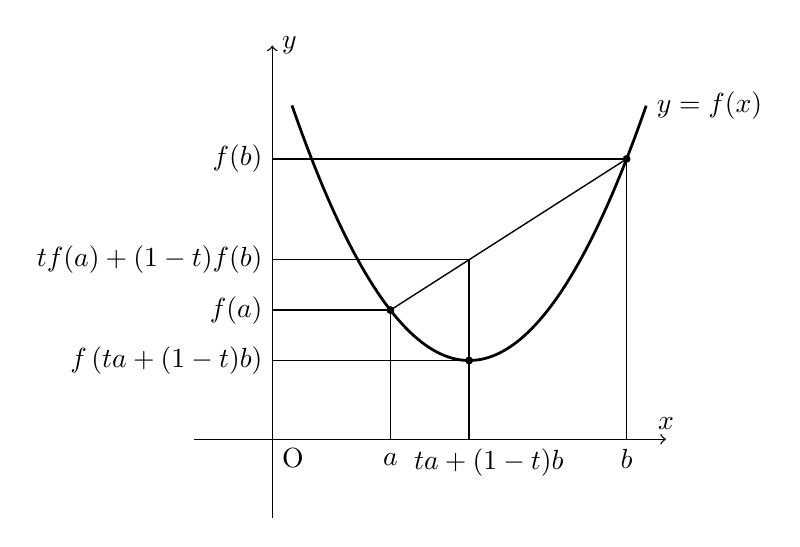
\begin{tikzpicture}
    \draw[->,line width=0.5pt] (-1,0)--(5,0) node[above]{$x$}; %x軸
    \draw[->,line width=0.5pt] (0,-1)--(0,5) node[right]{$y$}; %y軸
    \draw[line width=0.5pt] (0,3.56)--(4.5,3.56)--(4.5,0);
    \draw[line width=0.5pt] (0,2.28)--(2.5,2.28)--(2.5,0); 
    \draw[line width=0.5pt] (0,1.64)--(1.5,1.64)--(1.5,0);
    \draw[line width=0.5pt] (0,1)--(2.5,1); 
    \draw[line width=0.5pt] (1.5,1.64)--(4.5,3.56); 
    \draw (0,0) node[below right] {O}; %原点
    \draw (0,3.56) node[left] {$f(b)$};
    \draw (0,2.28) node[left] {$tf(a)+(1-t)f(b)$};
    \draw (0,1.64) node[left] {$f(a)$};
    \draw (0,1) node[left] {$f\left(ta+(1-t)b\right)$};
    \draw (1.5,-0.06) node[below] {$a$};
    \draw (2.75,0) node[below] {$ta+(1-t)b$};
    \draw (4.5,0) node[below] {$b$};
    \draw[samples=100,domain=0.25:4.75,line width=1pt] plot(\x,0.64*\x*\x-3.2*\x+5) node[right] {$y=f(x)$}; 
    \fill (1.5,1.64) circle (0.05); 
    \fill (2.5,1) circle (0.05); 
    \fill (4.5,3.56) circle (0.05); 
  \end{tikzpicture}
%\includegraphics[width=160pt]{4.2.2.a.png}
\end{center}
同様にして、関数$f:D(f) \rightarrow \mathbb{R}$が、$\forall a,b \in I\forall t \in (0,1)$に対し、次式が成り立つとき、
\begin{align*}
f\left( ta + (1 - t)b \right) \geq tf(a) + (1 - t)f(b)
\end{align*}
この関数$f$はその区間$I$で上への凸、上への凸関数などという。また、次式が成り立つとき、
\begin{align*}
f\left( ta + (1 - t)b \right) > tf(a) + (1 - t)f(b)
\end{align*}
この関数$f$はその区間$I$で上への狭義凸関数などという。
\end{dfn}
\begin{dfn}
関数$f$が下への凸関数である、または、上への凸関数であるとき、その関数$f$は凸関数であるという。同様にして、関数$f$が下への狭義凸関数である、または、上への狭義凸関数であるとき、その関数$f$は狭義凸関数であるという。
\end{dfn}
\begin{thm}\label{4.2.2.16}
$I \subseteq D(f) \subseteq \mathbb{R}$なる区間$I$で関数$f:D(f) \rightarrow \mathbb{R}$の2階導関数$\partial^{2}f$が存在するとき、次のことは同値である。
\begin{itemize}
\item
  その関数$f$はその区間$I$で下への凸関数である。
\item
  $a < x < b$かつ$a,b,x \in I$なる実数たち$a$、$b$、$x$が次式を満たす。
\begin{align*}
\frac{f(x) - f(a)}{x - a} \leq \frac{f(b) - f(a)}{b - a} \leq \frac{f(b) - f(x)}{b - x}
\end{align*}
\item
  その1階導関数$\partial f$はその区間$I$上で単調増加する。
\item
  $\partial^{2}f|\mathrm{int}I \geq 0$が成り立つ。
\end{itemize}
また、同様に次のことが同値である。
\begin{itemize}
\item
  その関数$f$はその区間$I$で上への凸関数である。
\item
  $a < x < b$かつ$a,b,x \in I$なる実数たち$a$、$b$、$x$が次式を満たす。
\begin{align*}
\frac{f(x) - f(a)}{x - a} \geq \frac{f(b) - f(a)}{b - a} \geq \frac{f(b) - f(x)}{b - x}
\end{align*}
\item
  その1階導関数$\partial f$はその区間$I$上で単調減少する。
\item
  $\partial^{2}f|\mathrm{int}I \leq 0$が成り立つ。
\end{itemize}
\end{thm}
\begin{proof}
$I \subseteq D(f) \subseteq \mathbb{R}$なる区間$I$で関数$f:D(f) \rightarrow \mathbb{R}$の2階導関数$\partial^{2}f$が存在するとする。$\partial^{2}f|\mathrm{int}I \geq 0$が成り立つとき、Taylorの定理より次式が成り立つような実数$c$が区間$(a,x) \cup (x,a)$に存在するのであった。
\begin{align*}
f(x) = f(a) + (x - a)\partial f(x) + \frac{(x - a)^{2}}{2}\partial^{2}f(c)
\end{align*}
ここで、$c \in I$が成り立ち仮定より$\partial^{2}f(c) \geq 0$が成り立つので、$\frac{(x - a)^{2}}{2}\partial^{2}f(c) \geq 0$が成り立つ。したがって、次のようになる。
\begin{align*}
f(x) = f(a) + (x - a)\partial f(x) + \frac{(x - a)^{2}}{2}\partial^{2}f(c) \geq f(a) + (x - a)\partial f(x)
\end{align*}
これにより、$\forall a,b \in I\forall t \in (0,1)$に対し、$x = ta + (1 - t)b$とおくと、次のようになる。
\begin{align*}
\left\{ \begin{matrix}
f(a) \geq f(x) + (a - x)\partial f(x) \\
f(b) \geq f(x) + (b - x)\partial f(x) \\
\end{matrix} \right.\ 
\end{align*}
したがって、次のようになる。
\begin{align*}
&\quad \left\{ \begin{matrix}
tf(a) \geq tf(x) + t(a - x)\partial f(x) \\
(1 - t)f(b) \geq (1 - t)f(x) + (1 - t)(b - x)\partial f(x) \\
\end{matrix} \right.\ \\
&\Rightarrow tf(a) + (1 - t)f(b) \geq tf(x) + t(a - x)\partial f(x) + (1 - t)f(x) + (1 - t)(b - x)\partial f(x)\\
&\Leftrightarrow tf(a) + (1 - t)f(b) \geq (t + 1 - t)f(x) + (ta - tx + b - x - tb + tx)\partial f(x)\\
&\Leftrightarrow tf(a) + (1 - t)f(b) \geq f(x) + (ta - tx + b - x - tb + tx)\partial f(x)
\end{align*}
ここで、次のようになることから、
\begin{align*}
ta - tx + b - x - tb + tx &= ta - t\left( ta + (1 - t)b \right) + b - \left( ta + (1 - t)b \right) - tb + t\left( ta + (1 - t)b \right)\\
&= ta - t^{2}a - tb + t^{2}b + b - ta - b + tb - tb + t^{2}a + tb - t^{2}b\\
&= t^{2}a - t^{2}a + ta - ta + t^{2}b - t^{2}b + tb - tb + tb - tb + b - b = 0
\end{align*}
次のようになる。
\begin{align*}
\left\{ \begin{matrix}
f(a) \geq f(x) + (a - x)\partial f(x) \\
f(b) \geq f(x) + (b - x)\partial f(x) \\
\end{matrix} \right. &\Rightarrow tf(a) + (1 - t)f(b) \geq f(x) + 0\partial f(x)\\
&\Leftrightarrow tf(a) + (1 - t)f(b) \geq f\left( ta + (1 - t)b \right)
\end{align*}
これにより、その関数$f$はその区間$I$で下への凸関数である。\par
逆に、$a < x < b$とし、$t = \frac{x - b}{a - b}$とおくと、$0 < t < 1$で次のようになり
\begin{align*}
t = \frac{x - b}{a - b} &\Leftrightarrow t(a - b) = x - b\\
&\Leftrightarrow ta + b - tb = x\\
&\Leftrightarrow ta + (1 - t)b = x
\end{align*}
その関数$f$はその区間$I$で下への凸関数であるならそのときに限り、$\forall a,b \in I\forall t \in (0,1)$に対し、$a \neq b$が成り立つなら、$tf(a) + (1 - t)f(b) \geq f(x)$が成り立つのであったので、したがって、次のようになる。
\begin{align*}
\frac{x - b}{a - b}f(a) + \left( 1 - \frac{x - b}{a - b} \right)f(b) \geq f(x) &\Leftrightarrow \frac{x - b}{a - b}f(a) + \frac{a - b - x + b}{a - b}f(b) \geq f(x)\\
&\Leftrightarrow \frac{x - b}{a - b}f(a) + \frac{x - a}{b - a}f(b) \geq f(x)
\end{align*}
ここで、次のようになることから、
\begin{align*}
f(x) \leq \frac{x - b}{a - b}f(a) + \frac{x - a}{b - a}f(b) &\Leftrightarrow f(x) - f(a) \leq \frac{x - b}{a - b}f(a) + \frac{x - a}{b - a}f(b) - \frac{a - b}{a - b}f(a)\\
&\Leftrightarrow f(x) - f(a) \leq \frac{x - b - a + b}{a - b}f(a) + \frac{x - a}{b - a}f(b)\\
&\Leftrightarrow f(x) - f(a) \leq - \frac{x - a}{b - a}f(a) - \frac{x - a}{b - a}f(b)\\
&\Leftrightarrow \frac{f(x) - f(a)}{x - a} \leq \frac{f(b) - f(a)}{b - a}\\
f(x) \leq \frac{x - b}{a - b}f(a) + \frac{x - a}{b - a}f(b) &\Leftrightarrow f(x) - f(b) \leq \frac{x - b}{a - b}f(a) + \frac{x - a}{b - a}f(b) - \frac{b - a}{b - a}f(b)\\
&\Leftrightarrow f(x) - f(b) \leq \frac{x - b}{a - b}f(a) + \frac{x - a - b + a}{b - a}f(b)\\
&\Leftrightarrow f(x) - f(b) \leq - \frac{x - b}{b - a}f(a) - \frac{x - b}{b - a}f(b)\\
&\Leftrightarrow \frac{f(x) - f(b)}{x - b} \geq \frac{f(b) - f(a)}{b - a}
\end{align*}
したがって、次式が成り立つ。
\begin{align*}
\frac{f(x) - f(a)}{x - a} \leq \frac{f(b) - f(a)}{b - a} \leq \frac{f(b) - f(x)}{b - x}
\end{align*}\par
また、$a < x < b$かつ$a,b,x \in I$なる実数たち$a$、$b$、$x$が次式を満たすとき、
\begin{align*}
\frac{f(x) - f(a)}{x - a} \leq \frac{f(b) - f(a)}{b - a} \leq \frac{f(b) - f(x)}{b - x}
\end{align*}
$x = a + \delta$、$x = b + \varepsilon$とおくと、次式のように書かれることができ、
\begin{align*}
\frac{f(a + \delta) - f(a)}{\delta} \leq \frac{f(b) - f(a)}{b - a} \leq \frac{f(b + \varepsilon) - f(b)}{\varepsilon}
\end{align*}
$\delta,\varepsilon \rightarrow 0$とすれば、次のようになる。
\begin{align*}
\lim_{\scriptsize \begin{matrix}
\delta \rightarrow 0 \\
\delta \neq 0 \\
\end{matrix}}\frac{f(a + \delta) - f(a)}{\delta} \leq \frac{f(b) - f(a)}{b - a} \leq \lim_{\scriptsize \begin{matrix}
\varepsilon \rightarrow 0 \\
\varepsilon \neq 0 \\
\end{matrix}}\frac{f(b + \varepsilon) - f(b)}{\varepsilon}
\end{align*}
微分の定義より、$\forall a,b \in I$に対し、$a < b$が成り立つなら、次式が成り立つ。
\begin{align*}
\partial f(a) \leq \frac{f(b) - f(a)}{b - a} \leq \partial f(b)
\end{align*}
これにより、その1階導関数$\partial f$はその区間$I$上で単調増加する。\par
上記の関数の増減の議論より、これが成り立つならそのときに限り、$\partial^{2}f|\mathrm{int}I \geq 0$が成り立つ。\par
以上より、次のことは同値であることが示された。
\begin{itemize}
\item
  その関数$f$はその区間$I$で下への凸関数である。
\item
  $a < x < b$かつ$a,b,x \in I$なる実数たち$a$、$b$、$x$が次式を満たす。
\begin{align*}
\frac{f(x) - f(a)}{x - a} \leq \frac{f(b) - f(a)}{b - a} \leq \frac{f(b) - f(x)}{b - x}
\end{align*}
\item
  その1階導関数$\partial f$はその区間$I$上で単調増加する。
\item
  $\partial^{2}f|\mathrm{int}I \geq 0$が成り立つ。
\end{itemize}
同様にして、次のことが同値であることが示される。
\begin{itemize}
\item
  その関数$f$はその区間$I$で上への凸関数である。
\item
  $a < x < b$かつ$a,b,x \in I$なる実数たち$a$、$b$、$x$が次式を満たす。
\begin{align*}
\frac{f(x) - f(a)}{x - a} \geq \frac{f(b) - f(a)}{b - a} \geq \frac{f(b) - f(x)}{b - x}
\end{align*}
\item
  その1階導関数$\partial f$はその区間$I$上で単調減少する。
\item
  $\partial^{2}f|\mathrm{int}I \leq 0$が成り立つ。
\end{itemize}
\end{proof}
\begin{thm}\label{4.2.2.17}
$I \subseteq D(f) \in \mathbb{R}$なる区間$I$で関数$f:D(f) \rightarrow \mathbb{R}$の2階導関数$\partial^{2}f$が存在するとき、$\partial^{2}f|\mathrm{int}I > 0$が成り立つなら、次のことが成り立つ\footnote{これをうまく応用すれば、最大値、最小値を求めることができますが、まだ、厳密に議論するには予備知識が不足しているので、もうしばらく待っててください。}。
\begin{itemize}
\item
  $\forall a,x \in I$に対し、$x \neq a$が成り立つなら、次式が成り立つ。
\begin{align*}
f(x) > f(a) + (x - a)\partial f(a)
\end{align*}
\item
  その関数$f$はその区間$I$で下への狭義凸関数である。
\item
  $a < x < b$かつ$a,b,x \in I$なる実数たち$a$、$b$、$x$が次式を満たす。
\begin{align*}
\frac{f(x) - f(a)}{x - a} < \frac{f(b) - f(a)}{b - a} < \frac{f(b) - f(x)}{b - x}
\end{align*}
\end{itemize}
同様に、$\partial^{2}f|\mathrm{int}I < 0$が成り立つなら、次のことが成り立つ。
\begin{itemize}
\item
  $\forall a,x \in I$に対し、$x \neq a$が成り立つなら、次式が成り立つ。
\begin{align*}
f(x) < f(a) + (x - a)\partial f(a)
\end{align*}
\item
  その関数$f$はその区間$I$で上への狭義凸関数である。
\item
  $a < x < b$かつ$a,b,x \in I$なる実数たち$a$、$b$、$x$が次式を満たす。
\begin{align*}
\frac{f(x) - f(a)}{x - a} > \frac{f(b) - f(a)}{b - a} > \frac{f(b) - f(x)}{b - x}
\end{align*}
\end{itemize}
\end{thm}
\begin{proof}
$I \subseteq D(f) \in \mathbb{R}$なる区間$I$で関数$f:D(f) \rightarrow \mathbb{R}$の2階導関数$\partial^{2}f$が存在するとき、$\partial^{2}f|\mathrm{int}I > 0$が成り立つなら、Taylorの定理より次式が成り立つような実数$c$が区間$(a,x) \cup (x,a)$に存在するのであった。
\begin{align*}
f(x) = f(a) + (x - a)\partial f(x) + \frac{(x - a)^{2}}{2}\partial^{2}f(c)
\end{align*}
ここで、$c \in I$が成り立ち仮定より$\partial^{2}f(c) > 0$が成り立つので、$\frac{(x - a)^{2}}{2}\partial^{2}f(c) > 0$が成り立つ。したがって、次のようになる。
\begin{align*}
f(x) = f(a) + (x - a)\partial f(x) + \frac{(x - a)^{2}}{2}\partial^{2}f(c) > f(a) + (x - a)\partial f(x)
\end{align*}
これにより、$\forall a,x \in I$に対し、$x \neq a$が成り立つなら、$f(x) > f(a) + (x - a)\partial f(a)$が成り立つ。\par
これにより、$\forall a,b \in I\forall t \in (0,1)$に対し、$x = ta + (1 - t)b$とおくと、次のようになり、
\begin{align*}
\left\{ \begin{matrix}
f(a) > f(x) + (a - x)\partial f(x) \\
f(b) > f(x) + (b - x)\partial f(x) \\
\end{matrix} \right. &\Leftrightarrow \left\{ \begin{matrix}
tf(a) > tf(x) + t(a - x)\partial f(x) \\
(1 - t)f(b) > (1 - t)f(x) + (1 - t)(b - x)\partial f(x) \\
\end{matrix} \right.\ \\
&\Rightarrow tf(a) + (1 - t)f(b) > tf(x) + t(a - x)\partial f(x) \\
&\quad + (1 - t)f(x) + (1 - t)(b - x)\partial f(x)\\
&\Leftrightarrow tf(a) + (1 - t)f(b) > (t + 1 - t)f(x) \\
&\quad + (ta - tx + b - x - tb + tx)\partial f(x)\\
&\Leftrightarrow tf(a) + (1 - t)f(b) > f(x) + (ta - tx + b - x - tb + tx)\partial f(x)
\end{align*}
ここで、次のようになることから、
\begin{align*}
ta - tx + b - x - tb + tx &= ta - t\left( ta + (1 - t)b \right) + b - \left( ta + (1 - t)b \right) - tb + t\left( ta + (1 - t)b \right)\\
&= ta - t^{2}a - tb + t^{2}b + b - ta - b + tb - tb + t^{2}a + tb - t^{2}b\\
&= t^{2}a - t^{2}a + ta - ta + t^{2}b - t^{2}b + tb - tb + tb - tb + b - b = 0
\end{align*}
次のようになる。
\begin{align*}
\left\{ \begin{matrix}
f(a) > f(x) + (a - x)\partial f(x) \\
f(b) > f(x) + (b - x)\partial f(x) \\
\end{matrix} \right. &\Rightarrow tf(a) + (1 - t)f(b) > f(x) + 0\partial f(x)\\
&\Leftrightarrow tf(a) + (1 - t)f(b) > f\left( ta + (1 - t)b \right)
\end{align*}
これにより、その関数$f$はその区間$I$で下への狭義凸関数である。\par
逆に、$a < b$とし$ta + (1 - t)b = x$とおくと、その関数$f$はその区間$I$で下への狭義凸関数であるならそのときに限り、$\forall a,b \in I\forall t \in (0,1)$に対し、$a \neq b$が成り立つなら、$tf(a) + (1 - t)f(b) > f(x)$が成り立つ。ここで、関係$a < x < b$が成り立つことに注意すれば、次のようになり、
\begin{align*}
ta + (1 - t)b = x &\Leftrightarrow ta + b - tb = x\\
&\Leftrightarrow t(a - b) = x - b \Leftrightarrow t = \frac{x - b}{a - b}
\end{align*}
したがって、次のようになる。
\begin{align*}
\frac{x - b}{a - b}f(a) + \left( 1 - \frac{x - b}{a - b} \right)f(b) > f(x) &\Leftrightarrow \frac{x - b}{a - b}f(a) + \frac{a - b - x + b}{a - b}f(b) > f(x)\\
&\Leftrightarrow \frac{x - b}{a - b}f(a) + \frac{x - a}{b - a}f(b) > f(x)
\end{align*}
ここで、次のようになることから、
\begin{align*}
f(x) < \frac{x - b}{a - b}f(a) + \frac{x - a}{b - a}f(b) &\Leftrightarrow f(x) - f(a) < \frac{x - b}{a - b}f(a) + \frac{x - a}{b - a}f(b) - \frac{a - b}{a - b}f(a)\\
&\Leftrightarrow f(x) - f(a) < \frac{x - b - a + b}{a - b}f(a) + \frac{x - a}{b - a}f(b)\\
&\Leftrightarrow f(x) - f(a) < - \frac{x - a}{b - a}f(a) - \frac{x - a}{b - a}f(b)\\
&\Leftrightarrow \frac{f(x) - f(a)}{x - a} < \frac{f(b) - f(a)}{b - a}\\
f(x) < \frac{x - b}{a - b}f(a) + \frac{x - a}{b - a}f(b) &\Leftrightarrow f(x) - f(b) < \frac{x - b}{a - b}f(a) + \frac{x - a}{b - a}f(b) - \frac{b - a}{b - a}f(b)\\
&\Leftrightarrow f(x) - f(b) < \frac{x - b}{a - b}f(a) + \frac{x - a - b + a}{b - a}f(b)\\
&\Leftrightarrow f(x) - f(b) < - \frac{x - b}{b - a}f(a) - \frac{x - b}{b - a}f(b)\\
&\Leftrightarrow \frac{f(x) - f(b)}{x - b} > \frac{f(b) - f(a)}{b - a}
\end{align*}
したがって、次式が成り立つ。
\begin{align*}
\frac{f(x) - f(a)}{x - a} < \frac{f(b) - f(a)}{b - a} < \frac{f(b) - f(x)}{b - x}
\end{align*}\par
$\partial^{2}f|\mathrm{int}I > 0$が成り立つなら、次のことが成り立つ。
\begin{itemize}
\item
  $\forall a,x \in I$に対し、$x \neq a$が成り立つなら、次式が成り立つ。
\begin{align*}
f(x) > f(a) + (x - a)\partial f(a)
\end{align*}
\item
  その関数$f$はその区間$I$で下への狭義凸関数である。
\item
  $a < x < b$かつ$a,b,x \in I$なる実数たち$a$、$b$、$x$が次式を満たす。
\begin{align*}
\frac{f(x) - f(a)}{x - a} < \frac{f(b) - f(a)}{b - a} < \frac{f(b) - f(x)}{b - x}
\end{align*}
\end{itemize}\par
同様にして、$\partial^{2}f|\mathrm{int}I < 0$が成り立つなら、次のことが成り立つことも示される。
\begin{itemize}
\item
  $\forall a,x \in I$に対し、$x \neq a$が成り立つなら、次式が成り立つ。
\begin{align*}
f(x) < f(a) + (x - a)\partial f(a)
\end{align*}
\item
  その関数$f$はその区間$I$で上への狭義凸関数である。
\item
  $a < x < b$かつ$a,b,x \in I$なる実数たち$a$、$b$、$x$が次式を満たす。
\begin{align*}
\frac{f(x) - f(a)}{x - a} > \frac{f(b) - f(a)}{b - a} > \frac{f(b) - f(x)}{b - x}
\end{align*}
\end{itemize}
\end{proof}
\begin{thm}\label{4.2.2.18}
$I = [ a,b] \subseteq D(f) \in \mathbb{R}$なる区間$I$で関数$f:D(f) \rightarrow \mathbb{R}$の2階導関数$\partial^{2}f$が存在するとき、$\partial^{2}f|I > 0$が成り立つかつ、$f(a)f(b) < 0$が成り立つなら、その関数$f$はその区間$\mathrm{int}I$で$f(c) = 0$が成り立つような実数$c$をただ1つもつ。\par
このような実数$c$をその関数$f$のその区間$I$での零点などという。
\end{thm}
\begin{proof}
$I = [ a,b] \subseteq D(f) \in \mathbb{R}$なる区間$I$で関数$f:D(f) \rightarrow \mathbb{R}$の2階導関数$\partial^{2}f$が存在するとき、$\partial^{2}f|I > 0$が成り立つかつ、$f(a)f(b) < 0$が成り立つなら、その関数$f$はその区間$I$で微分可能でありその区間$I$で連続であるかつ、仮定より次のようになるので、
\begin{align*}
f(a)f(b) < 0 &\Leftrightarrow \left( f(a) > 0 \land f(b) < 0 \right) \vee \left( f(a) < 0 \land f(b) > 0 \right)\\
&\Leftrightarrow f(b) < 0 < f(a) \vee f(a) < 0 < f(b)\\
&\Leftrightarrow f(a) \lessgtr 0 \lessgtr f(b)
\end{align*}
したがって、中間値の定理よりその関数$f$はその区間$\mathrm{int}I$で$f(c) = 0$が成り立つような実数$c$をもつ。\par
ここで、$f\left( c \right) = f\left( d \right) = 0$が成り立つような$a < c < d < b$なる実数たち$c$、$d$が複数存在するとする。このとき、明らかに、次式が成り立つような実数たち$s$、$t$が区間$(0,1)$に存在し、
\begin{align*}
c = sa + \left( 1 - s \right)d,\ \ d = tc + \left( 1 - t \right)b
\end{align*}
$\partial^{2}f|I > 0$が成り立つので、その関数$f$はその区間$I$で下に狭義凸関数である。したがって、次のようになる。
\begin{align*}
\left\{ \begin{matrix}
f\left( c \right) = f\left( d \right) = 0 \\
c = sa + \left( 1 - s \right)d \\
d = tc + \left( 1 - t \right)b \\
f\left( sa + \left( 1 - s \right)d \right) < sf(a) + \left( 1 - s \right)f\left( d \right) \\
f\left( tc + \left( 1 - t \right)b \right) < tf\left( c \right) + \left( 1 - t \right)f(b) \\
\end{matrix} \right. &\Leftrightarrow \left\{ \begin{matrix}
0 < sf(a) + \left( 1 - s \right)f\left( d \right) \\
0 = f\left( c \right) = f\left( sa + \left( 1 - s \right)d \right) \\
0 < \left( 1 - t \right)f(b) \\
0 = f\left( d \right) = f\left( tc + \left( 1 - t \right)b \right) \\
\end{matrix} \right.\\
&\Rightarrow \left\{ \begin{matrix}
0 < sf(a) \\
0 < \left( 1 - t \right)f(b) \\
\end{matrix} \right.\\
&\Leftrightarrow \left\{ \begin{matrix}
0 < f(a) \\
0 < f(b) \\
\end{matrix} \right.\\
&\Rightarrow f(a)f(b) > 0
\end{align*}
これは仮定$f(a)f(b) < 0$に矛盾する。\par
よって、その関数$f$はその区間$\mathrm{int}I$で$f(c) = 0$が成り立つような実数$c$をただ1つもつ。
\end{proof}
\begin{thm}[Newtonの逐次近似法]\label{4.2.2.19}
$I = [ a,b] \subseteq D(f) \in \mathbb{R}$なる区間$I$で関数$f:D(f) \rightarrow \mathbb{R}$の2階導関数$\partial^{2}f$が存在し、$\partial^{2}f|I > 0$が成り立つかつ、$f(a)f(b) < 0$が成り立つとし、$f\left( x_{1} \right) > 0かつx_{1} \in \mathrm{int}I$なる実数$x_{1}$を1つとり、$\forall n \in \mathbb{N}$に対し、実数$x_{n + 1}$が次式のように定義されるとする。
\begin{align*}
x_{n + 1} = x_{n} - \frac{f\left( x_{n} \right)}{\partial f\left( x_{n} \right)}
\end{align*}
このとき、その実数列$\left( x_{n} \right)_{n \in \mathbb{N}}$は単調増加するか、単調減少しその区間$I$におけるただ1つの零点に収束する。これによって、その区間$I$における方程式$f(x) = 0$の解が数値的に求められることができる。この方法をNewtonの逐次近似法、Newton法などという。
\begin{center}
  \begin{tikzpicture}
    \draw[->,line width=0.5pt] (-1,0)--(5,0) node[above]{$x$}; %x軸
%   \draw[->,line width=0.5pt] (0,-1)--(0,5) node[right]{$p'$}; %y軸
    \draw[line width=0.5pt] (4,0)--(4,3.44)--(1.47,0)--(1.47,0.89)--(0.24,0);
    \draw (0,0) node[above left] {$\lim_{n\to \infty } x_n$};
    \draw (4,0) node[below] {$x_1 $};
    \draw (1.47,0) node[below] {$x_2 $};
    \draw (0.24,0) node[below] {$x_3 $};
    \draw[samples=100,domain=-1:5,line width=1pt] plot(\x,{2*exp(\x/4 ) -2} ) node[right] {$y=f\left( x\right) $}; 
    \fill (0,0) circle (0.05); 
    \fill (4,3.44) circle (0.05); 
    \fill (1.47,0.89) circle (0.05); 
  \end{tikzpicture}
%\includegraphics[width=160pt]{4.2.2.b.png}
\end{center}
\end{thm}
\begin{proof}
$I = [ a,b] \subseteq D(f) \in \mathbb{R}$なる区間$I$で関数$f:D(f) \rightarrow \mathbb{R}$の2階導関数$\partial^{2}f$が存在し、$\partial^{2}f|I > 0$が成り立つかつ、$f(a)f(b) < 0$が成り立つとし、$f\left( x_{1} \right) > 0$かつ$x_{1} \in \mathrm{int}I$なる実数$x_{1}$を1つとり、$\forall n \in \mathbb{N}$に対し、実数$x_{n + 1}$が次式のように定義されるとする。
\begin{align*}
x_{n + 1} = x_{n} - \frac{f\left( x_{n} \right)}{\partial f\left( x_{n} \right)}
\end{align*}\par
このとき、$\mu \in I$かつ$\partial f(\mu) = 0$が成り立つような実数$\mu$が考えられると、$\partial^{2}f|I > 0$が成り立つので、定理\ref{4.2.2.17}より$\forall x \in I$に対し、$x \neq \mu$が成り立つなら、次式が成り立つ。
\begin{align*}
f(x) > f(\mu) + (x - \mu)\partial f(\mu) = f(\mu)
\end{align*}
これにより、$f(\mu) = \min{V\left( f \middle| I \right)}$が成り立つ。\par
ここで、仮定より次のようになるので、
\begin{align*}
f(a)f(b) < 0 &\Leftrightarrow \left( f(a) > 0 \land f(b) < 0 \right) \vee \left( f(a) < 0 \land f(b) > 0 \right)\\
&\Leftrightarrow f(b) < 0 < f(a) \vee f(a) < 0 < f(b)\\
&\Leftrightarrow f(a) \lessgtr 0 \lessgtr f(b)
\end{align*}
次式のように集合$J$を定め
\begin{align*}
J = \left\{ x \in I \middle| f(x) \geq 0 \right\}
\end{align*}
$\mu \in J$と仮定すると、$f(a) < 0 < f(b)$のとき、$f(a) < 0 \leq f(\mu)$が成り立つが、これは$f(\mu) = \min{V\left( f \middle| I \right)}$が成り立つことに矛盾する。$f(a) < 0 < f(b)$のときも同様にして示される。\par
したがって、$\mu \notin J$が成り立ち、したがって、$\forall\mu \in I$に対し、$\partial f(\mu) = 0$が成り立つなら、$\mu \notin J$も成り立つ。対偶律より$\forall x \in I$に対し、$x \in J$が成り立つなら、$\partial f(x) \neq 0$が成り立つ。\par
ここで、上記の議論より、$\partial^{2}f|I > 0$が成り立つかつ、$f(a)f(b) < 0$が成り立つなら、その関数$f$はその区間$\mathrm{int}I$で零点$c$をただ1つもつのであった。\par
ここで、$f(a) > 0$のとき、関係$a < c < b$より$a < d < c$かつ$f(d) \leq 0$となるような実数$d$が存在するとすると、$f(d) = 0$のときは$d \in \mathrm{int}I$よりその関数$f$がその区間$\mathrm{int}I$で零点$c$をただ1つもつことに矛盾するので、$f(d) < 0$が成り立つことになり、その関数$f$は区間$[ a,d]$で連続で$f(d) < 0 < f(a)$が成り立つので、中間値の定理より$f\left( c' \right) = 0$となる実数$c'$がその区間$[ a,d]$に存在し、さらに、$f(d) < f\left( c' \right) = 0 < f(a)$より$a \neq c'$かつ$d \neq c'$が成り立つことになり$a < c' < d < c$が成り立つ。これにより、その関数$f$の零点$c'$がその実数$c$とは別にその区間$\mathrm{int}I$で存在することになるが、その関数$f$がその区間$\mathrm{int}I$で零点$c$をただ1つもつことに矛盾する。\par
以上より、ある実数$d$が開区間$(a,c)$に存在して$f(d) \leq 0$が成り立つことがいえない、即ち、$\forall x \in (a,c)$に対し、$f(x) > 0$が成り立つ。同様にして、$\forall x \in (c,b)$に対し、$f(x) < 0$が成り立つことも示される。\par
ここで、次式たちが成り立つことにより
\begin{align*}
I = \left\{ a \right\} \sqcup (a,c) \sqcup \left\{ c \right\} \sqcup (c,b) \sqcup \left\{ b \right\},\\
\forall x \in \left\{ a \right\}\left[ f(x) > 0 \right],\ \ 
\forall x \in (a,c)\left[ f(x) > 0 \right],\\
\forall x \in \left\{ c \right\}\left[ f(x) = 0 \right],\ \ 
\forall x \in (c,b)\left[ f(x) < 0 \right],\ \ 
\forall x \in \left\{ b \right\}\left[ f(x) < 0 \right]
\end{align*}
$J = \left\{ a \right\} \sqcup (a,c) \sqcup \left\{ c \right\} = [ a,c]$が成り立つ。\par
また、$\partial f|J \geq 0$が成り立つと仮定しよう。$\forall x \in I$に対し、$x \in J$が成り立つなら、$\partial f(x) \neq 0$が成り立つのであったので、$\partial f\partial f(x) = 0$が成り立たなく$\partial f(x) > 0$が成り立つことになり、その区間$[ a,c]$で平均値の定理より次式が成り立つような実数$c'$が区間$\mathrm{int}[ a,c] = (a,c)$に存在する。
\begin{align*}
\partial f\left( c' \right) = \frac{f(c) - f(a)}{c - a}
\end{align*}
したがって、次のようになる。
\begin{align*}
\partial f\left( c' \right) = \frac{f(c) - f(a)}{c - a} &\Leftrightarrow f(c) - f(a) = (c - a)\partial f\left( c' \right)\\
&\Leftrightarrow f(c) = f(a) + (c - a)\partial f\left( c' \right)
\end{align*}
ここで、$f(c) = 0$より次のようになる。
\begin{align*}
\partial f\left( c' \right) = \frac{f(c) - f(a)}{c - a} &\Leftrightarrow 0 = f(a) + (c - a)\partial f\left( c' \right)\\
&\Leftrightarrow (a - c)\partial f\left( c' \right) = f(a)
\end{align*}
ここで、$c' \in (a,c) \subset J$が成り立ち$\partial f\left( c' \right) > 0$が成り立つかつ、$a < c$が成り立つので、次式が得られる。
\begin{align*}
0 > (a - c)\partial f\left( c' \right) = f(a)
\end{align*}
これは仮定の$f(a) > 0$が成り立つことに矛盾する。したがって、$\forall x \in J$に対し、$\partial f(x) < 0$が成り立つ。\par
ここで、仮定より、$f\left( x_{1} \right) > f(c) = 0$より$x_{1} \neq c$が成り立つことに注意すれば、明らかに$a < x_{1} < c$が成り立つ。\par
$n = k$のとき、$a < x_{k} < c$が成り立つと仮定しよう。このとき、$f(a) > 0$のとき、$\forall x \in (a,c)$に対し、$f(x) > 0$が成り立つのであったので、上記の議論より$f\left( x_{k} \right) > 0$かつ$\partial f\left( x_{k} \right) < 0$が成り立つので、$- \frac{f\left( x_{k} \right)}{\partial f\left( x_{k} \right)} > 0$が成り立つ。$n = k + 1$のとき、その実数列$\left( x_{n} \right)_{n \in \mathbb{N}}$の定義より次式が成り立ち、
\begin{align*}
x_{k + 1} = x_{k} - \frac{f\left( x_{k} \right)}{\partial f\left( x_{k} \right)}
\end{align*}
$- \frac{f\left( x_{k} \right)}{\partial f\left( x_{k} \right)} > 0$が成り立つので、$x_{k} < x_{k + 1}$が成り立つ。さらに、仮定より$a < x_{k}$が成り立つことに注意すれば、$a < x_{k} < x_{k + 1}$が成り立つ。また、仮定より$\forall x \in I$に対し、$\partial^{2}f(x) > 0$が成り立つので、$c \in I$より$\partial^{2}f(c) > 0$が成り立ち、$f\left( x_{k} \right) > f(c) = 0$より$x_{k} \neq c$が成り立つことに注意すれば、上記の定理より$f(c) > f\left( x_{k} \right) + \left( c - x_{k} \right)\partial f\left( x_{k} \right)$が成り立つ。\par
ここで、$f\left( x_{k} \right) > 0$かつ$\partial f\left( x_{k} \right) < 0$が成り立つことに注意すれば、次のようになる。
\begin{align*}
0 = f(c) > f\left( x_{k} \right) + \left( c - x_{k} \right)\partial f\left( x_{k} \right) &\Leftrightarrow 0 = \frac{f(c)}{\partial f\left( x_{k} \right)} < \frac{1}{\partial f\left( x_{k} \right)}\left( f\left( x_{k} \right) + \left( c - x_{k} \right)\partial f\left( x_{k} \right) \right)\\
&\Leftrightarrow 0 = \frac{f(c)}{\partial f\left( x_{k} \right)} < \frac{f\left( x_{k} \right)}{\partial f\left( x_{k} \right)} + c - x_{k}\\
&\Leftrightarrow 0 = \frac{f(c)}{\partial f\left( x_{k} \right)} < c - \left( x_{k} - \frac{f\left( x_{k} \right)}{\partial f\left( x_{k} \right)} \right)\\
&\Leftrightarrow 0 = \frac{f(c)}{\partial f\left( x_{k} \right)} < c - x_{k + 1} \Rightarrow x_{k + 1} < c
\end{align*}
以上より、$a < x_{k} < x_{k + 1} < c$が成り立つ。\par
数学的帰納法によって$\forall n \in \mathbb{N}$に対し、$a < x_{n} < x_{n + 1} < c$が成り立つ。これにより、その実数列$\left( x_{n} \right)_{n \in \mathbb{N}}$は上に有界であるかつ、単調増加するので、$\lim_{n \rightarrow \infty}x_{n} \in \mathbb{R}$が成り立つ。この実数$\lim_{n \rightarrow \infty}x_{n}$は少なくとも$a < \lim_{n \rightarrow \infty}x_{n} \leq c$が成り立っているので、$\lim_{n \rightarrow \infty}x_{n} \in J$が成り立ち、$\forall x \in I$に対し、$x \in J \Rightarrow \partial f(x) \neq 0$が成り立つのであったので、$\partial f\left( \lim_{n \rightarrow \infty}x_{n} \right) \neq 0$が成り立つことに注意すれば、$n \rightarrow \infty$のとき、次のようになる。
\begin{align*}
\lim_{n \rightarrow \infty}x_{n + 1} = \lim_{n \rightarrow \infty}\left( x_{n} - \frac{f\left( x_{n} \right)}{\partial f\left( x_{n} \right)} \right) &\Leftrightarrow \lim_{n \rightarrow \infty}x_{n} = \lim_{n \rightarrow \infty}x_{n} - \lim_{n \rightarrow \infty}\frac{f\left( x_{n} \right)}{\partial f\left( x_{n} \right)}\\
&\Leftrightarrow 0 = - \frac{f\left( \lim_{n \rightarrow \infty}x_{n} \right)}{\partial f\left( \lim_{n \rightarrow \infty}x_{n} \right)}\\
&\Leftrightarrow f\left( \lim_{n \rightarrow \infty}x_{n} \right) = 0
\end{align*}
ここで、その関数$f$がその区間$\mathrm{int}I$で零点$c$をただ1つもつのであったので、$c = \lim_{n \rightarrow \infty}x_{n}$が成り立つ。\par
よって、その実数列$\left( x_{n} \right)_{n \in \mathbb{N}}$は単調増加しその区間$I$におけるただ1つの零点に収束する。$f(a) < 0$のときも同様にして示される。
\end{proof}
%\hypertarget{lhuxf4pitalux306eux5b9aux7406}{%
\subsubsection{l'Hôpitalの定理}%\label{lhuxf4pitalux306eux5b9aux7406}}
\begin{thm}[l'Hôpitalの定理]\label{4.2.2.20}
ある区間$I$を用いた$I \subseteq D(f) \subseteq \mathbb{R}$かつ$I \subseteq D(g) \subseteq \mathbb{R}$なる関数たち$f:D(f) \rightarrow \mathbb{R}$、$g:D(g) \rightarrow \mathbb{R}$が、実数$a$を用いて$\mathfrak{a} =a$のとき、区間$I$がその実数$aの\varepsilon 近傍U(a,\varepsilon)$で、$\mathfrak{a = \infty}$のとき、その区間$I$が上に有界でない区間で、$\mathfrak{a} = - \infty$のとき、その区間$I$が下に有界でない区間であるとして、その区間$I$で微分可能であるとする。
\begin{itemize}
\item
  次式たちが成り立つかつ、
\begin{align*}
\lim_{x \rightarrow \mathfrak{a}}{f(x)} = \lim_{x \rightarrow \mathfrak{a}}{g(x)} = 0,\ \ \forall x \in I\left[ \partial g(x) \neq 0 \right]
\end{align*}
極限$\lim_{x \rightarrow \mathfrak{a}}{\frac{\partial f}{\partial g}(x)}$が振動しなければ、次式が成り立つ。
\begin{align*}
\lim_{x \rightarrow \mathfrak{a}}{\frac{f}{g}(x)} = \lim_{x \rightarrow \mathfrak{a}}{\frac{\partial f}{\partial g}(x)}
\end{align*}
\item
  次式たちが成り立つかつ、
\begin{align*}
\lim_{x \rightarrow \mathfrak{a}}{g(x)} = \infty,\ \ \forall x \in I\left[ \partial g(x) \neq 0 \right]
\end{align*}
極限$\lim_{x \rightarrow \mathfrak{a}}{\frac{\partial f}{\partial g}(x)}$が振動しなければ、次式が成り立つ。
\begin{align*}
\lim_{x \rightarrow \mathfrak{a}}{\frac{f}{g}(x)} = \lim_{x \rightarrow \mathfrak{a}}{\frac{\partial f}{\partial g}(x)}
\end{align*}
\end{itemize}
この定理をl'Hôpitalの定理という\footnote{
ここで少し反例を。ただ、高校数学の内容であるもののまだ述べられていない内容も含まれますので、目を通す程度でOKです。\par
\begin{itemize}
\item
$\lim_{x \rightarrow \mathfrak{a}}{f(x)} = \lim_{x \rightarrow \mathfrak{a}}{g(x)} = 0$が成り立っていない場合として、例えば、$f(x)=\cos x$、$g(x)=x$のときが挙げられる。$x\rightarrow +0$で$f(x)=\cos x\rightarrow 1$、$g(x)=x \rightarrow 0$となっているものの、$f'(x)=-\sin x$、$g'(x)=1$なので、次のようになる。
\begin{align*}
\lim_{x\rightarrow +0}{\frac{f(x)}{g(x)}} &=\lim_{x\rightarrow +0}{\frac{\cos x}{x}} =\infty, \\
\lim_{x\rightarrow +0}{\frac{f'(x)}{g'(x)}} &=\lim_{x\rightarrow +0}{(-\sin x)} =0
\end{align*}
\item
極限$\lim_{x \rightarrow \mathfrak{a}}{\frac{\partial f}{\partial g}(x)}$が振動してしまっている場合として、例えば、$f(x)=x^2 \sin \frac{1}{x}$、$g(x)=x$のときが挙げられる。$x\rightarrow +0$で、$0\leq \sin \frac{1}{x} \leq 1$かつ$x^2 \rightarrow 0$なので、はさみうちの原理より$f(x)=x^2 \sin \frac{1}{x}\rightarrow 0$、$g(x)\rightarrow 0$となっている。ここで、$x\rightarrow +0$で、$0\leq \sin \frac{1}{x} \leq 1$なので、はさみうちの原理より次のようになる。
\begin{align*}
\lim_{x\rightarrow +0}{\frac{f(x)}{g(x)}} =\lim_{x\rightarrow +0}{x\sin \frac{1}{x}} =0
\end{align*}
一方で、$f'(x)=2x\sin \frac{1}{x} -\cos \frac{1}{x}$、$g'(x)=1$なので、次のようになる。
\begin{align*}
\lim_{x\rightarrow +0}{\frac{f'(x)}{g'(x)}} &=\lim_{x\rightarrow +0}{\left( 2x\sin \frac{1}{x} -\cos \frac{1}{x}\right) } \\
&=\lim_{\frac{1}{x} \rightarrow \infty }{\left( 2x\sin \frac{1}{x} -\cos \frac{1}{x}\right) } =\mathrm{indefinite} 
\end{align*}
\item
$\forall x \in I\left[ \partial g(x) \neq 0 \right]$が成り立っていない場合として、例えば、$f(x)=\frac{1}{2} +\frac{1}{4}\sin 2x$、$g(x)=f(x) e^{\sin x}$のときが挙げられる。このとき、$x\rightarrow \infty $で$-1\leq \sin 2x $と追い出しの原理より$f(x),g(x)\rightarrow \infty $となる。もちろん$x\rightarrow \infty $で$e^{\sin x} =\mathrm{indefinite}$なので、次のようになる。
\begin{align*}
\lim_{x\rightarrow \infty }{\frac{f(x)}{g(x)}} =\lim_{x\rightarrow \infty }{\frac{1}{e^{\sin x} }}=\mathrm{indefinite}
\end{align*}
ここで、次のようになるので、
\begin{align*}
f'(x) &= \frac{1}{2} +\frac{1}{2} \cos 2x ={\cos }^2 x\\
g'(x) &= f'(x) e^{\sin x} +f(x) e^{\sin x} \cos x\\
&=\cos x\left( \cos x e^{\sin x} +g(x) \right)
\end{align*}
$\forall n\in \mathbb{Z} $に対し、$\cos \left( \frac{\pi }{2} +n\pi \right) =0$なので、$g' \left( \frac{\pi }{2} +n\pi \right) =0$となっている。ゆえに、上に有界でないどの区間でもある$x$が存在して、$g'(x)=0$となっている。このとき、$-1\leq \sin x, \cos x$に注意すれば、$-\frac{1}{e} \leq \cos x e^{\sin x}$なので、次のようになる。
\begin{align*}
0&\leq \left| \frac{\cos x}{\cos x e^{\sin x} +g(x)} \right| \\
&\leq \frac{1}{\left| \cos xe^{\sin x} +g(x)\right| } \\
&\leq \frac{1}{-\frac{1}{e} +g(x)}
\end{align*}
$x\rightarrow \infty $で$\frac{1}{-\frac{1}{e} +g(x)} \rightarrow 0$となっている。はさみうちの原理よりしたがって、次のようになる。
\begin{align*}
\lim_{x\rightarrow \infty }{\frac{f'(x)}{g'(x)}} =\lim_{x\rightarrow \infty }{\frac{\cos x}{\cos x e^{\sin x} +g(x)} }=0
\end{align*}
\end{itemize}
}。
\end{thm}
\begin{proof}
ある区間$I$を用いた$I \subseteq D(f) \subseteq \mathbb{R}$かつ$U\left( a,\gamma + \delta \right) \subseteq D(g) \subseteq \mathbb{R}$なる関数たち$f:D(f) \rightarrow \mathbb{R}$、$g:D(g) \rightarrow \mathbb{R}$が、実数$a$を用いて$\mathfrak{a} =a$のとき、区間$I$がその実数$a$の$\gamma + \delta$近傍$U\left( a,\gamma + \delta \right)$で、$\mathfrak{a = \infty}$のとき、その区間$I$が上に有界でない区間で、$\mathfrak{a = - \infty}$のとき、その区間$I$が下に有界でない区間であるとして、その区間$I$で微分可能であるとする。\par
次式たちが成り立つかつ、
\begin{align*}
\lim_{x \rightarrow \mathfrak{a}}{f(x)} = \lim_{x \rightarrow \mathfrak{a}}{g(x)} = 0,\ \ \forall x \in I\left[ \partial g(x) \neq 0 \right]
\end{align*}
極限$\lim_{x \rightarrow \mathfrak{a}}{\frac{\partial f}{\partial g}(x)}$が振動しないとき、$\mathfrak{a} =a$かつ$a < x$のとき、$x = a + \gamma + \delta$なる正の実数$\gamma + \delta$を用いてCauchyの平均値の定理より次式が成り立つような実数$c$が$(a,x) \subset U\left( a,\gamma + \delta \right)$なる区間$(a,x)$に存在する。
\begin{align*}
\frac{f(x) - f(a)}{g(x) - g(a)} = \frac{f}{g}(x) = \frac{\partial f}{\partial g}(c)
\end{align*}
ここで、$\gamma + \delta \rightarrow 0$とすると、$0 < c - a < \gamma + \delta$より$c - a \rightarrow 0$となり、したがって、次式が成り立つ。
\begin{align*}
\lim_{\gamma + \delta \rightarrow 0}{\frac{f}{g}(x)} = \lim_{\gamma + \delta \rightarrow 0}{\frac{\partial f}{\partial g}(c)} = \lim_{c - a \rightarrow 0}{\frac{\partial f}{\partial g}(c)} = \lim_{x \rightarrow a}{\frac{\partial f}{\partial g}(x)}
\end{align*}
$a > x$のときも同様にして示される。\par
$\mathfrak{a = \infty}$のとき、$x \rightarrow \infty$とすれば、$\frac{1}{x} \rightarrow + 0$となるので、次式が成り立つ。
\begin{align*}
\lim_{x \rightarrow \infty}{\frac{f}{g}(x)} = \lim_{\frac{1}{x} \rightarrow + 0}{\frac{f}{g}\left( \frac{1}{\frac{1}{x}} \right)} = \lim_{\frac{1}{x} \rightarrow + 0}{\frac{\partial f}{\partial g}\left( \frac{1}{\frac{1}{x}} \right)} = \lim_{x \rightarrow \infty}{\frac{\partial f}{\partial g}(x)}
\end{align*}
$\mathfrak{a = - \infty}$のときも同様にして示される。\par
また、次式たちが成り立つかつ、
\begin{align*}
\lim_{x \rightarrow \mathfrak{a}}{g(x)} = \infty,\ \ \forall x \in I\left[ \partial(g)(x) \neq 0 \right]
\end{align*}
極限$\lim_{x \rightarrow \mathfrak{a}}{\frac{\partial f}{\partial g}(x)}$が振動しないとき、$\mathfrak{a} =a$かつ$a < x$のとき、$a + \gamma < x = a + \gamma + \delta$なる正の実数たち$\gamma$、$\delta$を用いてCauchyの平均値の定理より次式が成り立つような実数$c$が$\left( a + \gamma,x \right) \subset U\left( a,\gamma + \delta \right)$なる区間$\left( a + \gamma,x \right)$に存在する。
\begin{align*}
\frac{f(x) - f\left( a + \gamma \right)}{g(x) - g\left( a + \gamma \right)} = \frac{\partial f}{\partial g}(c)
\end{align*}
ここで、仮定の$\lim_{x \rightarrow a}{g(x)} = \infty$より$\forall\varepsilon \in \mathbb{R}^{+}\exists\delta \in \mathbb{R}^{+}$に対し、$0 < |x - a| < \delta \Rightarrow \varepsilon < g(x)$が成り立つ。これにより、$0 < g(x)$が成り立つので、次のようになる。
\begin{align*}
\frac{f(x) - f\left( a + \gamma \right)}{g(x) - g\left( a + \gamma \right)} = \frac{\partial f}{\partial g}(c) &\Leftrightarrow f(x) - f\left( a + \gamma \right) = \frac{\partial f}{\partial g}(c)\left( g(x) - g\left( a + \gamma \right) \right)\\
&\Leftrightarrow \frac{f(x) - f\left( a + \gamma \right)}{g\left( a + \gamma \right)} = \frac{\partial f}{\partial g}(c)\frac{g(x) - g\left( a + \gamma \right)}{g\left( a + \gamma \right)}\\
&\Leftrightarrow \frac{f(x)}{g\left( a + \gamma \right)} - \frac{f}{g}\left( a + \gamma \right) = \frac{\partial f}{\partial g}(c)\left( \frac{g(x)}{g\left( a + \gamma \right)} - 1 \right)\\
&\Leftrightarrow \frac{f}{g}\left( a + \gamma \right) = \frac{f(x)}{g\left( a + \gamma \right)} + \frac{\partial f}{\partial g}(c) - \frac{\partial f}{\partial g}(c)\frac{g(x)}{g\left( a + \gamma \right)}
\end{align*}
$\lim_{x \rightarrow a}{\frac{\partial f}{\partial g}(x)} \in \mathbb{R}$のとき、$\lim_{x \rightarrow a}{\frac{\partial f}{\partial g}(x)} = \alpha$とおく。$\gamma + \delta \rightarrow 0$とすると、$0 < c - a < \gamma + \delta$より$c - a \rightarrow 0$となり、したがって、次式が成り立つ。
\begin{align*}
\lim_{\gamma + \delta \rightarrow 0}{\frac{\partial f}{\partial g}(c)} = \lim_{c - a \rightarrow 0}{\frac{\partial f}{\partial g}(c)} = \lim_{c \rightarrow a}{\frac{\partial f}{\partial g}(c)} = \alpha
\end{align*}
これにより、$\forall\varepsilon' \in \mathbb{R}^{+}\exists\delta' \in \mathbb{R}^{+}$に対し、$0 < \gamma + \delta < \delta' \Leftrightarrow 0 < \gamma < \gamma + \delta < \delta' \Rightarrow \left| \frac{\partial f}{\partial g}(c) - \alpha \right| < \varepsilon'$が成り立つ。関数$\frac{\partial f}{\partial g}:(a,x) \rightarrow \mathbb{R}$は上に有界となるので、$\forall a + \delta_{0} \in (a,x)$に対し、次式が成り立つような正の実数$R$が存在する。
\begin{align*}
\left| \frac{\partial f}{\partial g}\left( a + \delta_{0} \right) \right| \leq R
\end{align*}
仮定の$\lim_{x \rightarrow a}{g(x)} = \infty$より、次のようになる。
\begin{align*}
\lim_{\gamma \rightarrow 0}\frac{f(x)}{g\left( a + \gamma \right)} &= \lim_{a + \gamma \rightarrow a}\frac{f\left( a + \gamma + \delta \right)}{g\left( a + \gamma \right)}\\
&= \lim_{a + \gamma \rightarrow a}{f\left( a + \gamma + \delta \right)}\lim_{a + \gamma \rightarrow a}\frac{1}{g\left( a + \gamma \right)}\\
&= f\left( a + \delta \right) \cdot 0 = 0\\
\lim_{\gamma \rightarrow 0}\frac{g(x)}{g\left( a + \gamma \right)} &= \lim_{a + \gamma \rightarrow a}\frac{g\left( a + \gamma + \delta \right)}{g\left( a + \gamma \right)}\\
&= \lim_{a + \gamma \rightarrow a}{g\left( a + \gamma + \delta \right)}\lim_{a + \gamma \rightarrow a}\frac{1}{g\left( a + \gamma \right)}\\
&= g\left( a + \delta \right) \cdot 0 = 0
\end{align*}
これにより、$\forall\varepsilon \in \mathbb{R}^{+}\exists\delta'' \in \mathbb{R}^{+}$に対し、$0 < \gamma < \delta'' \Rightarrow \left| \frac{f(x)}{g\left( a + \gamma \right)} \right| < \varepsilon''$が成り立つかつ、$\forall\varepsilon \in \mathbb{R}^{+}\exists\delta''' \in \mathbb{R}^{+}$に対し、$0 < \gamma < \delta''' \Rightarrow \left| \frac{g(x)}{g\left( a + \gamma \right)} \right| < \varepsilon'''$が成り立つ。以上より、$a < a + \gamma < x = a + \gamma + \delta$より$x \rightarrow a$とすれば、$\gamma \rightarrow 0$となり、$\forall\varepsilon \in \mathbb{R}^{+}$に対し、$0 < \gamma < \min\left\{ \delta',\delta'',\delta''' \right\} = \delta''''$なる実数$\delta''''$が存在して次式のようになる。
\begin{align*}
\left| \frac{f}{g}\left( a + \gamma \right) - \alpha \right| &= \left| \frac{f(x)}{g\left( a + \gamma \right)} + \frac{\partial f}{\partial g}(c) - \frac{\partial f}{\partial g}(c)\frac{g(x)}{g\left( a + \gamma \right)} - \alpha \right|\\
&\leq \left| \frac{f(x)}{g\left( a + \gamma \right)} \right| + \left| \frac{\partial f}{\partial g}(c) - \alpha \right| + \left| - \frac{\partial f}{\partial g}(c) \right|\left| \frac{g(x)}{g\left( a + \gamma \right)} \right|\\
&< \varepsilon'' + \varepsilon' + R\varepsilon''' = \varepsilon' + \varepsilon'' + R\varepsilon'''
\end{align*}
これにより、$0 < \gamma < \delta'''' \Leftrightarrow 0 < \left| a + \gamma - a \right| < \delta''''$が成り立つことに注意すれば、$\forall\varepsilon' + \varepsilon'' + R\varepsilon''' \in \mathbb{R}^{+}\exists\delta'''' \in \mathbb{R}^{+}$に対し、次式が成り立つ。
\begin{align*}
0 < \left| a + \gamma - a \right| < \delta'''' \Rightarrow \left| \frac{f}{g}\left( a + \gamma \right) - \alpha \right| < \varepsilon' + \varepsilon'' + R\varepsilon'''
\end{align*}
これにより、$\lim_{x \rightarrow a}{\frac{f}{g}(x)} = \alpha$が成り立つので、よって、次式が成り立つ。
\begin{align*}
\lim_{x \rightarrow a}{\frac{f}{g}(x)} = \lim_{x \rightarrow a}{\frac{\partial f}{\partial g}(x)}
\end{align*}\par
$\lim_{x \rightarrow a}{\frac{\partial f}{\partial g}(x)} = \infty$のとき、$\gamma + \delta \rightarrow 0$とすると、$0 < c - a < \gamma + \delta$より$c - a \rightarrow 0$となり、したがって、次式が成り立つ。
\begin{align*}
\lim_{\gamma + \delta \rightarrow 0}{\frac{\partial f}{\partial g}(c)} = \lim_{c - a \rightarrow 0}{\frac{\partial f}{\partial g}(c)} = \lim_{c \rightarrow a}{\frac{\partial f}{\partial g}(c)} = \infty
\end{align*}
これにより、$\forall\varepsilon \in \mathbb{R}^{+}\exists\delta' \in \mathbb{R}^{+}$に対し、次式が成り立つ。
\begin{align*}
0 < \gamma + \delta < \delta' \Leftrightarrow 0 < \gamma < \gamma + \delta < \delta' \Rightarrow \varepsilon < \frac{\partial f}{\partial g}(c)
\end{align*}
仮定の$\lim_{x \rightarrow a}{g(x)} = \infty$より、次のようになり、
\begin{align*}
\lim_{\gamma \rightarrow 0}\frac{f(x)}{g\left( a + \gamma \right)} &= \lim_{a + \gamma \rightarrow a}\frac{f\left( a + \gamma + \delta \right)}{g\left( a + \gamma \right)}\\
&= \lim_{a + \gamma \rightarrow a}{f\left( a + \gamma + \delta \right)}\lim_{a + \gamma \rightarrow a}\frac{1}{g\left( a + \gamma \right)}\\
&= f\left( a + \delta \right) \cdot 0 = 0\\
\lim_{\gamma \rightarrow 0}\frac{g(x)}{g\left( a + \gamma \right)} &= \lim_{a + \gamma \rightarrow a}\frac{g\left( a + \gamma + \delta \right)}{g\left( a + \gamma \right)}\\
&= \lim_{a + \gamma \rightarrow a}{g\left( a + \gamma + \delta \right)}\lim_{a + \gamma \rightarrow a}\frac{1}{g\left( a + \gamma \right)}\\
&= g\left( a + \delta \right) \cdot 0 = 0
\end{align*}
これにより、$\forall\varepsilon \in \mathbb{R}^{+}\exists\delta'' \in \mathbb{R}^{+}$に対し、次式が成り立つかつ、
\begin{align*}
0 < \gamma < \delta'' \Rightarrow \left| \frac{f(x)}{g\left( a + \gamma \right)} \right| < \varepsilon
\end{align*}
$\forall\varepsilon \in \mathbb{R}^{+}\exists\delta''' \in \mathbb{R}^{+}$に対し、次式が成り立つ。
\begin{align*}
0 < \gamma < \delta''' \Rightarrow \left| \frac{g(x)}{g\left( a + \gamma \right)} \right| < \varepsilon
\end{align*}
特に、$\exists\delta'' \in \mathbb{R}^{+}$に対し、次式が成り立つかつ、
\begin{align*}
0 < \gamma < \delta'' \Rightarrow - \frac{1}{2} \leq \frac{f(x)}{g\left( a + \gamma \right)}
\end{align*}
$\exists\delta''' \in \mathbb{R}^{+}$に対し、次式が成り立つようにすることができる。
\begin{align*}
0 < \gamma < \delta''' \Rightarrow \frac{1}{2} \leq 1 - \frac{g(x)}{g\left( a + \gamma \right)}
\end{align*}
以上より、$a < a + \gamma < x = a + \gamma + \delta$より$x \rightarrow a$とすれば、$\gamma \rightarrow 0$となり、$\forall\varepsilon \in \mathbb{R}^{+}$に対し、$0 < \gamma < \min\left\{ \delta',\delta'',\delta''' \right\} = \delta''''$なる実数$\delta''''$が存在して次式のようになる。
\begin{align*}
\frac{f}{g}\left( a + \gamma \right) = \frac{f(x)}{g\left( a + \gamma \right)} + \frac{\partial f}{\partial g}(c)\left( 1 - \frac{g(x)}{g\left( a + \gamma \right)} \right) > - \frac{1}{2} + \varepsilon \cdot \frac{1}{2} = \frac{\varepsilon - 1}{2}
\end{align*}
これにより、$0 < \gamma < \delta'''' \Leftrightarrow 0 < \left| a + \gamma - a \right| < \delta''''$が成り立つことに注意すれば、$\forall(2 + R)\varepsilon \in \mathbb{R}^{+}\exists\delta'''' \in \mathbb{R}^{+}$に対し、次式が成り立つ。
\begin{align*}
0 < \left| a + \gamma - a \right| < \delta'''' \Rightarrow \frac{\varepsilon - 1}{2} < \frac{f}{g}\left( a + \gamma \right)
\end{align*}
これにより、$\lim_{x \rightarrow a}{\frac{f}{g}(x)} = \infty$が成り立つので、よって、次式が成り立つ。
\begin{align*}
\lim_{x \rightarrow a}{\frac{f}{g}(x)} = \lim_{x \rightarrow a}{\frac{\partial f}{\partial g}(x)}
\end{align*}
$a > x$のときも同様にして示される。\par
$\mathfrak{a = \infty}$のとき、$x \rightarrow \infty$とすれば、$\frac{1}{x} \rightarrow + 0$となるので、次式が成り立つ。
\begin{align*}
\lim_{x \rightarrow \infty}{\frac{f}{g}(x)} = \lim_{\frac{1}{x} \rightarrow + 0}{\frac{f}{g}\left( \frac{1}{\frac{1}{x}} \right)} = \lim_{\frac{1}{x} \rightarrow + 0}{\frac{\partial f}{\partial g}\left( \frac{1}{\frac{1}{x}} \right)} = \lim_{x \rightarrow \infty}{\frac{\partial f}{\partial g}(x)}
\end{align*}
$\mathfrak{a = - \infty}$のときも同様にして示される。
\end{proof}
\begin{thebibliography}{50}
  \bibitem{1}
  杉浦光夫, 解析入門I, 東京大学出版社, 1985. 第34刷 p64-75 ISBN978-4-13-062005-5
  \bibitem{2}
  高橋淳也. "l'Hˆopital の定理とその注意点(解析学 A)". 東北大学. \url{http://www.math.is.tohoku.ac.jp/~junya/lecture/calculus/l'Hopital.pdf} (2021-2-19 取得)
\end{thebibliography}
\end{document}
